%%%%%%%%%%%%%%%%%%%%%%%%%%%%%%%%%%%%%%%%%%%%%%%%%%%%%%%%%%%%%%%%%%%%%%%%%%%%
% AGUJournalTemplate.tex: this template file is for articles formatted with LaTeX
%
% This file includes commands and instructions
% given in the order necessary to produce a final output that will
% satisfy AGU requirements, including customized APA reference formatting.
%
% You may copy this file and give it your
% article name, and enter your text.
%
%
% Step 1: Set the \documentclass
%
%

%% To submit your paper:
\documentclass[draft]{agujournal2019}
\usepackage{url} %this package should fix any errors with URLs in refs.
\usepackage{lineno}
\usepackage[inline]{trackchanges} %for better track changes. finalnew option will compile document with changes incorporated.
\usepackage{soul}
\linenumbers
\usepackage{graphicx}
\usepackage{amsmath,amsfonts,amsthm,bm}
\DeclareMathOperator{\tr}{Tr}
\usepackage{amssymb}
\usepackage[fleqn,tbtags]{mathtools}
\usepackage{tensor}
\usepackage{breakcites}
\usepackage{siunitx}
\usepackage{multirow}
\usepackage{xcolor}
\usepackage[super]{nth}
\usepackage[geometry]{ifsym}
\usepackage{multirow}
%\usepackage{epstopdf}

\renewcommand{\Re}{\operatorname{Re} } 
\renewcommand{\Im}{\operatorname{Im} } 

%%%%%%%
% As of 2018 we recommend use of the TrackChanges package to mark revisions.
% The trackchanges package adds five new LaTeX commands:
%
%  \note[editor]{The note}
%  \annote[editor]{Text to annotate}{The note}
%  \add[editor]{Text to add}
%  \remove[editor]{Text to remove}
%  \change[editor]{Text to remove}{Text to add}
%
% complete documentation is here: http://trackchanges.sourceforge.net/
%%%%%%%

\draftfalse

%% Enter journal name below.
%% Choose from this list of Journals:
%
% JGR: Atmospheres
% JGR: Biogeosciences
% JGR: Earth Surface
% JGR: Oceans
% JGR: Planets
% JGR: Solid Earth
% JGR: Space Physics
% Global Biogeochemical Cycles
% Geophysical Research Letters
% Paleoceanography and Paleoclimatology
% Radio Science
% Reviews of Geophysics
% Tectonics
% Space Weather
% Water Resources Research
% Geochemistry, Geophysics, Geosystems
% Journal of Advances in Modeling Earth Systems (JAMES)
% Earth's Future
% Earth and Space Science
% Geohealth
%
% ie, \journalname{Water Resources Research}
\linespread{1.6}
\journalname{JGR: Solid Earth}


\begin{document}

%% ------------------------------------------------------------------------ %%
%  Title
%
% (A title should be specific, informative, and brief. Use
% abbreviations only if they are defined in the abstract. Titles that
% start with general keywords then specific terms are optimized in
% searches)
%
%% ------------------------------------------------------------------------ %%

\title{Homogenization of hydraulically isolated porous thin layers in the absence of periodic heterogeneities for seismic reflectivity applications}

%% ------------------------------------------------------------------------ %%
%
%  AUTHORS AND AFFILIATIONS
%
%% ------------------------------------------------------------------------ %%

% Authors are individuals who have significantly contributed to the
% research and preparation of the article. Group authors are allowed, if
% each author in the group is separately identified in an appendix.)

% List authors by first name or initial followed by last name and
% separated by commas. Use \affil{} to number affiliations, and
% \thanks{} for author notes.
% Additional author notes should be indicated with \thanks{} (for
% example, for current addresses).

% Example: \authors{A. B. Author\affil{1}\thanks{Current address, Antartica}, B. C. Author\affil{2,3}, and D. E.
% Author\affil{3,4}\thanks{Also funded by Monsanto.}}

\authors{Edith Sotelo\affil{1}, Nicol\'{a}s D. Barbosa\affil{1}, Santiago G. Solazzi\affil{1}, J. Germ\'{a}n Rubino\affil{2}, Marco Favino\affil{1}, Klaus Holliger\affil{1} }


 \affiliation{1}{Institute of Earth Sciences, University of Lausanne, Lausanne, Switzerland }
 \affiliation{2}{CONICET, Centro Atómico Bariloche - CNEA, San Carlos de Bariloche, Argentina}
 %\affiliation{3}{Department of Earth Sciences, University of Geneva, Geneva, Switzerland}
% \affiliation{4}{Fourth Affiliation}

%(repeat as many times as is necessary)

%% Corresponding Author:
% Corresponding author mailing address and e-mail address:

% (include name and email addresses of the corresponding author.  More
% than one corresponding author is allowed in this LaTeX file and for
% publication; but only one corresponding author is allowed in our
% editorial system.)

% Example: \correspondingauthor{First and Last Name}{email@address.edu}

\correspondingauthor{Edith Sotelo}{edith.sotelogamboa@unil.ch}

%% Keypoints, final entry on title page.

%  List up to three key points (at least one is required)
%  Key Points summarize the main points and conclusions of the article
%  Each must be 100 characters or less with no special characters or punctuation and must be complete sentences

% Example:
% \begin{keypoints}
% \item	List up to three key points (at least one is required)
% \item	Key Points summarize the main points and conclusions of the article
% \item	Each must be 100 characters or less with no special characters or punctuation and must be complete sentences
% \end{keypoints}

\begin{keypoints}
\item We propose a procedure to homogenize isolated porous thin layers with non-periodic heterogenous structures.
\item This procedure modifies classical approaches to account for the boundary conditions induced by the isolating background.
\item Results shows that the corresponding effective moduli reproduce closely the P-wave reflectivities of the porous thin layer.


%\item 
\end{keypoints}

%% ------------------------------------------------------------------------ %%
%
%  ABSTRACT and PLAIN LANGUAGE SUMMARY
%
% A good Abstract will begin with a short description of the problem
% being addressed, briefly describe the new data or analyses, then
% briefly states the main conclusion(s) and how they are supported and
% uncertainties.

% The Plain Language Summary should be written for a broad audience,
% including journalists and the science-interested public, that will not have 
% a background in your field.
%
% A Plain Language Summary is required in GRL, JGR: Planets, JGR: Biogeosciences,
% JGR: Oceans, G-Cubed, Reviews of Geophysics, and JAMES.
% see http://sharingscience.agu.org/creating-plain-language-summary/)
%
%% ------------------------------------------------------------------------ %%


\begin{abstract}
Seismic-scale thin layers  of interest often present prominent mechanical and/or hydraulic contrasts with the embedding background and, hence, are important targets for seismic reflection studies. We consider a simple, yet realistic thin layer  model that consists of a stack of few porous and permeable beds with distinct fluid and rock properties that is embedded in a background deemed impermeable for the seismic frequency range.
Such model allows representing thin layers of interest that are relevant in subsurface applications.  
Moreover, an efficient way to study the reflectivity response of a porous thin layer is to employ its homogenized viscoelastic equivalent.
Classical poroelastic-to-viscoelastic homogenization  procedures of porous media with a deterministic arrangements of heterogeneities rely on the existence of a periodic heterogeneous structure, for example, an ensemble of beds that repeats sufficiently to ensure that its effective response is unaffected by external boundary conditions (BC). However the considered thin layer model does not present such periodicity and, therefore, the estimation of its effective viscoelastic moduli is inherently affected by the BC associated with the embedding background. Thus, we propose to account for the appropriate BC in the homogenization procedure. 
Classical homogenization methodologies perform oscillatory relaxation tests over a representative sample of the periodic structure, followed by the averaging of stress and strain components, which are then used to estimate the effective moduli. We adapt this procedure for our non-periodic thin layer model to incorporate the BC induced by the embedding background. To this end, we apply the oscillatory relaxation tests on a sample that includes part of the background while the averaging of stress and strain components is performed only over the thin layer section. To test the proposed method, we consider a thin layer embedded in impermeable half-spaces and that is composed by a stack of two porous sand beds, where the upper one is gas-saturated and the bottom one is water-saturated. Then, after estimating the thin layer effective moduli using the proposed homogenization procedure, we  calculate the P-wave reflectivities at the interface between the upper half-space and the thin layer effective representation. We compare these results against the ones obtained using the porous thin layer. 
Results show that the effective moduli obtained using the proposed methodology are able to closely reproduce the reflectivities of the porous thin layer in the seismic frequency range with errors below  4 \% . This methodology can be readily extended to porous thin layers presenting strongly heterogenous structures such as inclusions or fractures.
\end{abstract}

\section*{Plain Language Summary}
We focus on thin layers in the seismic scale embedded in impermeable background that are of interest for underground applications such as carbon sequestration or gas exploitation. The strong contrast in physical properties that, in many cases, these layers present in comparison to the background rock makes them suitable for seismic reflection studies. To this end, we use a simple model that is capable to depict thin layers of interest. In this representation the thin layer consists of a stack of few porous beds with distinct physical properties. Moreover, a simplified technique to study the seismic response of a porous medium is to use its effective equivalent. Nonetheless, traditional homogenization procedures of porous media with an ordered arrangement of heterogeneities rely on the existence of a repetitive unit, for instance, a stack of beds that repeats sufficiently so that the boundary conditions of the surrounding medium does not affect the estimation of the effective moduli. Since the considered thin layer model does not present a repetitive unit, we propose a homogenization methodology that modifies traditional procedures in order to incorporate the influence of the boundary conditions associated with the background on the estimation of the effective moduli, with the overall goal of reproducing the seismic reflection response of the porous thin layer. We test the proposed method using a thin layer composed of a stack of two sand beds. The results show that the corresponding effective moduli are capable to satisfactory reproduce the reflectivity response of the porous thin layer.

%% ------------------------------------------------------------------------ %%
%
%  TEXT
%
%% ------------------------------------------------------------------------ %%

%%% Suggested section heads:
% \section{Introduction}
%
% The main text should start with an introduction. Except for short
% manuscripts (such as comments and replies), the text should be divided
% into sections, each with its own heading.

% Headings should be sentence fragments and do not begin with a
% lowercase letter or number. Examples of good headings are:

% \section{Materials and Methods}
% Here is text on Materials and Methods.
%
% \subsection{A descriptive heading about methods}
% More about Methods.
%
% \section{Data} (Or section title might be a descriptive heading about data)
%
% \section{Results} (Or section title might be a descriptive heading about the
% results)
%
% \section{Conclusions}


\section{Introduction}
Quantitative interpretation of seismic reflection data is a valuable tool to characterize rock and fluid properties.
This is particular relevant for the characterization of small-scale geological features in comparison to the predominant wavelength such as seismic-scale thin beds. In this regard,
a layer is considered to be thin if the reflections  from the top and bottom interfaces cannot be individually resolved by the predominant wavelength. Such that their compounded effect manifests itself as a single seismic reflection signal  \cite{Widess1973}. This effect occurs when the layer thickness is equal to or smaller than a quarter of the dominant wavelength \cite{Widess1973, Kallweit1982}.
The corresponding threshold is known as the the tuning thickness and is characterized by an initial constructive interference of the reflection signals from the top and bottom interfaces that becomes destructive as the layer thickness decreases \cite{Bakke1998, Hamlyn2014}.
Pertinent applications of reflectivity studies on thin layers are, for instance,  the characterization of gas-bearing beds \cite<e.g.,>{Cichostepski2019, Shakir2022}
as well as the monitoring of carbon sequestration \cite<e.g.,>{Williams2012,Zhang2013}. In general, proposed methodologies to estimate thin layer properties are largely developed in the frequency domain \cite<e.g.,>{Puryear2008,Rubino2009a,Zhang2013, Romdhane2014, Huang2016} and they are mainly applied in a pure elastic framework. This approach is likely to affect the accuracy of the estimated properties since the elastic theory cannot account for fluid interactions in heterogenoues porous rocks.

Conversely, using  a poroelastic framework allows for an accurate physical description of heterogenous porous rocks saturated with different fluids as they are commonly encountered in thin layers of interest. In particular, evidence suggests that heterogenoues porelastic media
exhibit an effective viscoelastic behavior regarding attenuation and velocity dispersion in the seismic frequency range. \cite<e.g.,>{Pride2004, Carcione2006}. This dispersive behavior is the consequence of an energy dissipation phenomenon known as wave-induced fluid flow or WIFF \cite<e.g.,>{Muller2010} that occurs when a passing seismic wave generates pressure gradients between different parts of a poroelastic medium
that equilibrate by fluid flow.
For typical frequencies used in seismic experiments, WIFF occurs predominantly in the mesoscopicscale range \cite<e.g.,>{Pride2004, Muller2010}. This refers to  WIFF taking place  between  heterogeneities that are larger than the prevailing pore size  but smaller than the wavelength \cite<e.g.,>{Norris1993}. In this context, the substitution of a heterogeneous thin layer by its homogenized viscoelastic representation can be deemed as an efficient technique to study its seismic reflectivity. Indeed, published work
shows the applicability of the poroelastic-to-viscoelastic homogenization approach to frequency-dependent seismic reflection studies of thin layers. For instance, \citeA{Rubino2011} and \citeA{Rubino2011a} employ viscoelastic substitutes to represent thin sand layers with different patchy saturations of CO$_2$ to investigate the corresponding effects on zero-offset seismic reflection data as well as on
the variation of amplitudes for different incident angles. Similarly,
\citeA{He2020} use viscoelastic substitutes of thin fractured layers to investigate their effect on P-wave amplitude variation with respect to the incident angle and frequency. Moreover, \citeA{Jin2017} use an effective viscoelastic representation to replace a partially gas-saturated thin layer. This model is later used to estimate gas saturation and layer thickness from seismic amplitude variation with the incident angle and frequency.

The pioneering work of \citeA{White1975a} and \citeA{White1975} is one of the first to show the effective viscoelastic behavior of simple poroelastic composites saturated with gas and water. Specially, the periodic model of alternating  porous beds  \cite{White1975} has been used to represent thin layers. 
In this modeling approach, the porous thin layer is assumed to be embedded in an impermeable background and to consist of a stack of periodically-repeating alternating beds that are deemed poroelastic, homogeneous and isotropic. This hydraulically isolated thin layer model is useful to represent relevant scenarios for subsurface applications such as the case of a porous sandstone thin layer  surrounded by impervious shale \cite<e.g.,>{Torres-verdin2012,AbuEl-Ata2019}, or the scenario of a narrow fractured or damage zone,  embedded in impermeable intact rock \cite<e.g.,>{Caine1996, Mitchell2012}. Several studies have applied the aforementioned model to investigate the frequency-dependent reflectivity response of thin layers of interest. In this regard, this thin layer representation with alternating beds is convenient for testing the sensitivity of various poroelastic parameters as it allows the computation of its effective moduli by analytical means \cite<e.g.,>{Carcione2006, Krzikalla2011}.
For instance, \citeauthor{Quintal2009} \citeyear{Quintal2009, Quintal2011a}
%\citeA{Quintal2009} %and \citeA{Quintal2011a}
compare the frequency-dependent reflection coefficients at normal incidence of viscoelastic substitutes of thin layer models embedded in elastic background that consist of a stack of periodically-repeating
alternating porous sands with different rock and fluid properties. Whereas, \citeA{He2020} utilize a particular version of this model to represent a thin layer containing fractures. In this case, they consider that the thin layer is embedded in impervious shale and that one of its alternating beds represents a horizontal fracture with a much higher permeability, softer moduli and smaller thickness  than the other bed \cite{Brajanovski2005,Kong2013}. In their study, they use viscoelastic substitutes of these fractured thin layers to examine the effect of various saturating fluids and fracture properties on the variation of seismic amplitude as a function of the angle of incidence and frequency. Nonetheless, a general assumption in the homogenization of porous medium containing a deterministic heterogeneous structure is its periodicity, for example, an ensemble of beds that repeats a sufficient number of times so that its
effective behavior is, for practical purposes, unaffected by the boundary conditions (BC) induced by the surrounding rock. However, a more realistic and flexible model to depict a porous thin layer with an internal bedding structure is to consider a model consisting of a stack of few porous beds with distinct rock and fluid properties. However, in such case, BC induced by the background embedding the thin layer inherently affect the estimation of its effective moduli. While, classical homogenization procedures are not readily applicable to this type of thin layer models, the development of a suitable procedure has been largely unexplored.
%the homogenization of the proposed TPL representation with a finite number of beds and distinct properties has been largely unexplored. 
%Consequently, the implementation of appropriate BC in a homogenization procedure to find  
%the corresponding effective viscoelastic representation capable of reproducing the reflectivity response of such TPL model has not been widely investigated. 

In this work, we seek to alleviate this problem by proposing a method to homogenize a porous thin layer consisting of a stack of non-periodic beds and that is embedded in a background deemed impermeable for the frequencies of interest, with the overall goal of adequately predicting its reflectivity. Classical homogenization procedures of periodic poroelastic media apply oscillatory relaxation tests to a representative sample of the periodic structure. This is followed by the averaging of the stress and the strain components over the sample to estimate the effective moduli. We adapt this methodology to incorporate in the estimation of effective moduli the influence of the BC induced by the embedding background.
In the Methodology section, we describe this proposed homogenization procedure that presents the following central modifications with respect to classical methods. First, it applies the corresponding oscillatory tests to a sample that incorporates part of the background and a representative section of the 
thin layer and, second, it performs the averaging of stress and strain components only over the thin layer section in order to find its effective moduli. In the Resuls section, we
test the accuracy of proposed method considering a thin layer model that is embedded in impervious rock represented by elastic half-spaces and that consists of a stack of two  porous sand beds. We estimate the corresponding effective moduli by applying the proposed homogenization procedure to then calculate P-wave reflectivities at the interface between the upper half-space and the effective representation of the thin  layer. Finally, we compare these results against those obtained using the porous thin layer. In the Discussion section we include an analysis of the BC induced by the embedding background and we also examine the effect of the background permeability in the effective moduli  estimation.

% Under this scenario, the BC induced by the embedding background is likely to affect the estimation of the corresponding effective moduli. In this study, we assume that this embedding background behaves as an impermeable rock for the frequencies of interest, allowing the entrapment of fluids e.g., natural gas or carbon, within the thin layer. Considering an impermeable background is relevant to represent, for instance, thin permeable sandstone layers intercalated by imprevious shales \cite<e.g.,>{Torres-verdin2012,AbuEl-Ata2019}, as well as to depict an open fracture surrounded by a permeable damage zone, which are embedded in an impermeable background rock \cite<e.g.,>{Caine1996, Mitchell2012}. 
% Then, to find the viscoelastic equivalent of thin layers with a non-periodic bedding structure,
%we propose to incorporate the pertinent BC induced by such impermeable embedding background in a numerical homogenization procedure. 
%
% The proposed method proceed as follows,
%we  apply the oscillatory relaxation tests to a sample that includes part of the embedding background as well as the entire thickness of the thin layer.. 
%We also calculate reflectivities using the homogenized media applying a classical homogenization procedure over a TPL sample as shown in Figure \ref{fig.1}b.
%we assume a infinite horizontal TPL model that consists of a finite number of of beds that present distinct rock and fluid properties. As stated, we also assume that the rock surrounding the TPL is impermeable for the frequencies of interest so that it allows the entrapment of fluids e.g., natural gas or carbon, within the TPL (Figure \ref{fig.1}a). Then, we propose to incorporate the no-flow constraint in the homogenization procedure using twp approaches. In the first approach, we take a sample of the TPL and prescribe mathematically the no-flow condition at the pertinent TPL boundaries (Figure \ref{fig.1}b).  considered periodic. Evidently, this latter approach disregards the no-flow condition that the impermeable background prescribes on the TPL. In the methodology section we detail the different approaches to incorporate the no-flow condition in the homogenization of the considered TPL model. Specifically, we present these approaches as modified procedures of the homogenization methodology proposed by \cite{Favino2020}. After this, in the results section, 


\section{Theory and methods}
In this section we detail the proposed homogenization procedure to estimate the effective moduli of an infinite horizontal thin layer embedded in background that is deemed impermeable for the frequencies of interest.  
%We assume that this thin layer-background system is defined in $\mathbb R^2$. 
In more detail, we consider that the thin layer consists of a stack of few distinct beds which are poroelastic, homogeneous and isotropic (Figure \ref{fig.1}a). 
The proposed homogenization procedure is based on the to the classical treatment described in \citeA{Favino2020} but incorporates substantial modifications with regards to
the extent of the sample considered as well as the volume over which strain and stress components are averaged. For the proposed method, the sample includes part of the embedding background and the corresponding section of the thin layer. Then, after applying the oscillatory test, the averaging of stress and strains is performed only over the domain pertaining to the thin layer.
 These novel adaptations allows
incorporating the effect of the BC induced by the embedding background in the estimation of the effective moduli of the thin layer model considered. 
On the other hand, reflectivity computations using the proposed poroelastic thin layer model  and its corresponding effective viscoelastic equivalent are detailed in Appendices A and B, respectively. Before presenting the proposed homogenization procedure,
we detail theoretical aspects regarding the validity of the poroelastic-to-viscoelastic equivalence.

\begin{figure}[!ht]
\centering
        \includegraphics[ width= 120mm, height=70mm]{TPL_combined_sampleE.eps}
\caption{ (a) Example of a thin layer model consisting of a stack of four distinct poroelastic beds B1, B2, B3 and B4. This thin layer is embedded in impermeable background represented by the half-spaces $\Lambda_1$ and $\Lambda_2$, respectively. The light blue box represents a sample $\Omega_e$ used for the proposed homogenization procedure. (b) Enlarged view of the sample $\Omega_e = \Omega_p \, \cup \, \Omega_b$, where  $\Omega_p$ is a representative section of the thin layer and  $\Omega_b= \Omega_{b1}  \, \cup \, \Omega_{b2}$ is a portion of the background, with $\Omega_{b1} \subset \Lambda_1$ and $\Omega_{b2} \subset \Lambda_2$, respectively. $\Gamma$ denotes the boundaries of the  sample $\Omega_e$, with  $\Gamma = \Gamma_1^+ \cup \Gamma_1^- \cup \Gamma_3^+ \cup \Gamma_3^-$.
}
\label{fig.1}
\end{figure}

\subsection{Mesoscale fluid pressure diffusion}
WIFF occurs when a seismic wave propagating through a heterogeneous poroelastic medium creates
pressure gradients that equilibrate by fluid flow \cite{Muller2010}.
We focus on WIFF that occurs between mesoscale heterogeneities since this is particularly relevant for seismic applications. Mesoscale heterogeneities refer to those with a characteristic size $L_m$ that are larger than the pore size $L_p$ but smaller than the wavelength $\lambda_w$. Specifically, for thin layers consisting of a stack of beds, the size of the mesoscale heterogeneity is dictated by the thickness of such beds.
For sufficiently low frequencies $f$, WIFF is viscosity-dominated and, therefore, controlled by fluid pressure diffusion (FPD). The reference frequency that indicates the transition from viscous-dominated towards inertial-dominated WIFF is Biot's characteristic frequency $f_B$ \cite{Biot1956, Dutta1979}
\begin{linenomath*}
\begin{equation}\label{Eq.1}
f_B= \frac{1}{2 \pi} \frac{\eta \phi}{ \rho_f \kappa S },
\end{equation}
\end{linenomath*}
where $\phi$ is the porosity, $\kappa$  the static permeability, $\eta$, the fluid viscosity,  $\rho_f$ the fluid density, and $S$ the tortuosity of the pore space. The aforementioned considerations regarding scales and frequencies can be summarized as
\begin{linenomath*}
\begin{equation}\label{Eq.2}
\begin{split}
 L_p & \ll L_m \ll \lambda_w, \\
f & \ll f_B.
\end{split}
\end{equation}
\end{linenomath*}
It can be shown that the fluid pressure diffusion equation governing FPD stems from \citeauthor{Biot1941}'s \citeyear{Biot1941} quasi-static equations \cite{Dutta1979, Chandler1981, Norris1993}. The corresponding diffusion coefficient $D$  together with its characteristic diffusion length $L_d$ can be expressed as \cite{Norris1993}
\begin{linenomath*}
\begin{equation}\label{Eq.3}
\begin{split}
&D= \frac {\kappa} {\eta} \frac{M H_d}{H},\\
&L_d=\sqrt{\frac{D}{\omega}},
\end{split}
\end{equation}
\end{linenomath*}
where $M$ is Biot’s fluid storage modulus, $H_d$ and $H$ are the drained and undrained plane-wave moduli, respectively, and $\omega$ is the angular frequency $\omega = 2 \pi f$.
The required rock physical properties are
\begin{linenomath*}
\begin{equation}\label{Eq.4}
\begin{split}
& H_d = \lambda_d + 2 \mu, \\
& H = H_d + M \alpha ^2, \\
& \lambda_d= K_m - \frac{2}{3} \mu, \\
& \alpha =1-\frac{K_m}{K_s},\\
& M  =\left( \frac{\alpha-\phi}{K_s} +\frac{\phi}{K_f} \right)^{-1},
\end{split}
\end{equation}
\end{linenomath*}
where $\lambda_d$ is the the drained Lamé modulus, $\mu$ is the shear modulus, $\alpha$ is the Biot-Willis effective stress coefficient, $K_m$, $K_s$, and $K_f$ are the bulk moduli of the drained solid frame, the solid grains, and the pore fluid, respectively.

The characteristic diffusion length $L_d$ together with the size of the heterogeneity $L_m$, e.g., thickness of the beds in the thin layer, determine the relaxed and unrelaxed FPD regimes. The relaxed state occurs at sufficiently low frequencies, for which  $L_d \gg L_m$. In this regime, there is enough time for the pressure between the beds to equilibrate. Conversely, the unrelaxed state occurs at sufficiently high frequencies, for which $L_d \ll L_m$ and, consequently, there is insufficient time for pressure equilibration to take place and, hence, the different beds behave as are hydraulically isolated. A transition zone exists at intermediate frequencies, for which $L_d \approx L_m$.
This zone is associated with attenuation and dispersion of body waves due to viscous dissipation. The maximum dissipation energy is related to a characteristic transition frequency $f_c= \omega_c/2\pi$, which depends on the diffusion coefficient $D$ and the characteristic size of the heterogeneity $L_m$ \cite{Muller2006}
\begin{linenomath*}
\begin{equation}\label{Eq.5}
\omega_c \propto \frac{D}{(L_m)^2}.
\end{equation}
\end{linenomath*}

The described mesoscopic FPD process produces an effective viscoelastic behavior of the thin layer under consideration. In more detail, the respective frequency-dependent  moduli that describe such a viscoelastic material can be estimated by solving \citeauthor{Biot1941}'s \citeyear{Biot1941} quasi-static equations over a representative sample of the thin layer and then applying volume averaging of the inferred strains and stresses.

\subsection{Proposed homogenization procedure}
We consider a thin layer that consists of a stack of few poroelastic beds, e.g. B1, B2, B3 and B4, that is embedded in the half-spaces $\Lambda_1$ and $\Lambda_2$ which represent impermeable background (Figure \ref{fig.1}a). To find the effective viscoelastic moduli of the thin layer, we apply the homogenization procedure described below over a sample $\Omega_e = \Omega_p \,\cup \, \Omega_b$ (Figure \ref{fig.1}b), where $\Omega_p$ denotes a representative section of the thin  layer and $\Omega_b =\Omega_{b1}\, \cup \, \Omega_{b2}$ is a portion of the background, with $\Omega_{b1} \subset \Lambda_1$ and $\Omega_{b2} \subset \Lambda_2$, respectively. As already stated, this sampling strategy allows incorporating the boundary effects induced by the presence of the embedding background on the effective viscoelastic moduli.


\subsubsection{Governing equations}
We solve Biot's consolidation equations \cite{Biot1941, Biot1962} over a sample  $\Omega_e$ of the thin layer of interest (Figures \ref{fig.1}a and \ref{fig.1}b) for each of the oscillatory relaxation tests specified in equations
\eqref{Eq.8} to \eqref{Eq.11}. We express these equations in the solid displacement - pressure ($\bm{u}-p$) formulation in the frequency domain \cite{Quintal2011,Favino2020},  with $\bm{u} = \bm{u}(\bm{x}, \omega)$ and $p = p(\bm{x},\omega)$, where $\bm{x} \in \Omega_e$ is the position and $\omega \in F$ is the angular frequency, with $F =(0,W]$. 
\begin{linenomath*}
\begin{equation}\label{Eq.6}
\begin{split}
& - \nabla \cdot \, \bm{\sigma} = \bm{0}  \quad  \textrm{in} \quad \Omega_e \times F,  \\
& - i \, \alpha \nabla . \, \bm{u} -i \frac{p}{M} + \frac{1}{\omega} \,\nabla \, \cdot \, \left( \frac{\kappa}{\eta} \nabla p\right)  =0 \quad  \textrm{in} \quad \Omega_e \times F,
\end{split}
\end{equation}
\end{linenomath*}
where $\bm{\sigma}$ is the total stress, $i$ is the imaginary unit.

The constitutive equation relating the total stress $\bm{\sigma}$ to $\bm{u}$ and $p$ is
\begin{linenomath*}
\begin{equation}\label{Eq.7}
\begin{split}
& \bm{\sigma} =  2\mu \, \bm{\varepsilon} +  \left( \lambda_d \,  \tr( \bm{\varepsilon})\, - \alpha \,p \right) \bm{I}, \qquad \text{with}\\
& \bm{\varepsilon} = \frac{1}{2} \left( \nabla \,\bm{u} + ({\nabla  \bm{u}})^T  \right),
 \end{split}
\end{equation}
\end{linenomath*}
where $\bm{\varepsilon}$ is the strain tensor,
and $\bm{I}$ the identity tensor. 

 
\subsubsection{Oscillatory relaxation tests}
In this subsection we detail the BC for the oscillatory relaxation tests. 
Hereinafter, we assume a Cartesian coordinate system in $\mathbb R^2$ with the associated basis vectors $\bm{\hat x_1}$ and $\bm{\hat x_3}$ parallel to the horizontal and vertical Cartesian axes, respectively. We also
let the sample $\Omega_e$ be a quadrilateral with boundary $\Gamma = \Gamma_1^+ \cup \Gamma_1^- \cup \Gamma_3^+ \cup \Gamma_3^- $, where $\Gamma_1^+ $ and $\Gamma_1^- $ are opposite boundaries with outer normal vectors $\bm{\hat x_1}$ and $ -\bm{\hat x_1}$, respectively. Similarly, $\Gamma_3^+ $ and $\Gamma_3^- $ are opposite boundaries with outer normal vectors $\bm{\hat x_3}$ and $ -\bm{\hat x_3}$ (Figure \ref{fig.1}b). To simplify the notation, we let $ \bm{\hat n}$ be the outer normal vector
of $\Gamma$.

In the following, we define periodic BC for displacements ($\bm{u}$), pressure ($p$), tractions ($\bm{\sigma}\cdot \bm{\hat n} $) and fluid flux relative to the solid ($\frac{\kappa}{\eta} \nabla p \cdot \bm{\hat n}$). We apply three different sets of displacement BC corresponding to the vertical and horizontal compression as well as the shear oscillatory relaxation tests. Here, we let $\Delta u$ be a real displacement difference in the frequency domain.

For the vertical compressional test, the BC for displacements are
\begin{linenomath*}
\begin{equation}\label{Eq.8}
\begin{split}
&  \bm{u} \cdot \bm{\hat{x}_3} \, \vert_{\Gamma_3^-} - \bm{u}\cdot \bm{\hat{x}_3}\, \vert_{\Gamma_3^+} =- \Delta u, \\
&  \bm{u} \cdot \bm{\hat{x}_1}\, \vert_{\Gamma_3^-} - \bm{u} \cdot \bm{\hat{x}_1} \, \vert_{\Gamma_3^+} = 0, \\
& \bm{u}\,\vert_{\Gamma_1^+} - \bm{u}\,\vert_{\Gamma_1^-} = \bm{0},
\end{split}
\end{equation}
\end{linenomath*}

For the horizontal compressional test, the BC for displacements are
\begin{linenomath*}
\begin{equation}\label{Eq.9}
\begin{split}
& \bm{u} \cdot \bm{\hat{x}_1}\, \vert_{\Gamma_1^+}-\bm{u} \cdot \bm{\hat{x}_1}\, \vert_{\Gamma_1^-} = - \Delta u, \\
& \bm{u} \cdot \bm{\hat{x}_3} \vert_{\Gamma_1^+}- \bm{u} \cdot \bm{\hat{x}_3}\vert_{\Gamma_1^-} =  0,  \\
& \bm{u}\,\vert_{\Gamma_3^-}- \bm{u}\,\vert_{\Gamma_3^+} = \bm{0}.
\end{split}
\end{equation}
\end{linenomath*}

Finally, for the shear test, the BC for displacements are
\begin{linenomath*}
\begin{equation}\label{Eq.10}
\begin{split}
& \bm{u} \cdot \bm{\hat{x}_1}\,\vert_{\Gamma_3^+}- \bm{u} \cdot \bm{\hat{x}_1} \,\vert_{\Gamma_3^-} =\Delta u,\\
& \bm{u} \cdot \bm{\hat{x}_3}\,\vert_{\Gamma_3^+}- \bm{u} \cdot \bm{\hat{x}_3}\,\vert_{\Gamma_3^-} = 0, \\
& \bm{u}\,\vert_{\Gamma_1+}- \bm{u}\,\vert_{\Gamma_1^-} =\bm{0}.
\end{split}
\end{equation}
\end{linenomath*}

For all relaxation tests, the respective BC for pressure, tractions and fluid flux relative to the solid are
\begin{linenomath*}
\begin{equation}\label{Eq.11}
\begin{split}
& p\vert_{\Gamma_k^+}-p\vert_{\Gamma_k^-} =0, \\
& \left(\bm{\sigma}\cdot \bm{\hat n} \right)\, \vert_{\Gamma_k^+}-\left(\bm{\sigma}\cdot \bm{\hat n} \right)\, \vert_{\Gamma_k^-} = \bm{0},\\
&\left( \frac{\kappa}{\eta} \nabla p \cdot \bm{\hat n} \right) \, \vert_{\Gamma_k^+} -\left( \frac{\kappa}{\eta} \nabla p \cdot \bm{\hat n} \right) \, \vert_{\Gamma_k^-} = 0.
\end{split}
\end{equation}
\end{linenomath*}
where the subscript $k$ in $\Gamma_k^-$ and $\Gamma_k^+$ takes the value of 1 or 3 at a time to denote opposite boundaries.

\subsubsection{Effective viscoelastic moduli}
In this subsection, we detail the steps to obtain the effective viscoelastic moduli from the three oscillatory relaxation tests. The first step consists in computing the average of the  stress and strain components. However, this computation is only performed over the sub-domain of interest $\Omega_p \subset \Omega_e$. This is followed by an estimation of the effective viscoelastic moduli that best fit these values. In the following, we outline this procedure.

For every oscillatory test $t$ with $t = \{1,2,3\}$, we calculate, over the sub-domain $\Omega_p$, the average  of the stress components $\langle \sigma_{ij}^t \rangle_{\Omega_p}$ and of the respective strain components $\langle \varepsilon_{ij}^t \rangle_{\Omega_p}$, with $i=\{1,3\}$ and $j=\{1,3\}$. The corresponding average quantities $\langle \Box \rangle_{\Omega_p}$ are computed as
\begin{linenomath*}
\begin{equation}\label{Eq.12}
  \langle \Box \rangle_{\Omega_p} = \frac{1}{\vert \Omega_p \vert} \int_{\Omega_p} \Box \, d\Omega_p, \qquad \text{with} \quad  \vert \Omega_p \vert = \int_{\Omega_p}  d \Omega_p.
\end{equation}
\end{linenomath*}

In Voigt's notation, the average strain and stress is related by the homogenized stiffness matrix $\bm{C} = \bm{C} (\omega) $. We remark that the elements of $\bm{C}$  are  complex-valued and frequency-dependent stiffness coefficients and we write this strain--stress relationship in frequency domain as
\begin{linenomath*}
\begin{equation}\label{Eq.13}
 \begin{split}
 \begin{pmatrix}
 \langle \sigma_{11}^t\rangle \\
 \langle \sigma_{33}^t\rangle \\
  \langle\sigma_{13}^t\rangle \\
 \end{pmatrix}
 =
   \begin{pmatrix}
  C_{11} & C_{13} & C_{15} \\
  C_{13} & C_{33} & C_{35} \\
  C_{15} & C_{35} & C_{55}\\
 \end{pmatrix}
  \begin{pmatrix}
 \langle\varepsilon_{11}^t \rangle \\
 \langle \varepsilon_{33}^t \rangle \\
 2\, \langle \varepsilon_{13}^t \rangle \\
 \end{pmatrix}.
 \end{split}
\end{equation}
\end{linenomath*}
Using this constitutive equation, a least squares minimization procedure is performed to find the best-fitting values of the viscoelastic moduli \cite{Rubino2016}. The obtained homogenized moduli are used for reflectivity calculations as further explained in Appendix B.

%\subsection{Proposed homogenization procedure}
%For this procedure, we take a sample $\Omega_e = \Omega_b \,\cup\, \Omega$ (Figures \ref{fig.1}a and \ref{fig.1}c) that includes part of the background rock $\Omega_b = \Omega_{b1}\, \cup \, \Omega_{b2} $ and the same TPL subdomain $\Omega$ used for the traditional procedure. After this, we apply the relaxation oscillatory tests on the sample $\Omega_e$. However, to find the effective moduli, we perform the average of stress and strain components only over the domain of interest  $\Omega$. We detail in the following the modifications with respect to the classical homogenization method.
%
%\begin{enumerate}
%\setlength\itemsep{1em}
%\item Governing Equations
%
%We use the same governing equations as expressed by Equations \eqref{Eq.6} and \eqref{Eq.7}. However, now we apply them over the domain $\Omega_e$. Thus, these governing equations are now valid $ \forall \, \bm{x} \in \Omega_e$.
%\\
%
%\item Oscillatory relaxation tests
%
%For this case, we let $\Gamma$ be the boundary of $\Omega_e$ with  $\Gamma = \Gamma_1^+ \,\cup \,\Gamma_1^- \,\cup \,\Gamma_3^+ \, \cup \, \Gamma_3^- $ (Figure \ref{fig.1}c).
%For the oscillatory relaxation tests, we consider the same set of BC: Equations \eqref{Eq.8} to \eqref{Eq.11}. 
%\\
%
%\item Homogenized viscoelastic moduli
%
%For each oscillatory relaxation test, we perform the averaging of stress and strain components as specified by Equation \eqref{Eq.12} over the subdomain of interest $\Omega \,\subset \, \Omega_e$. Finally, we find the viscoelastic moduli of $\Omega$, using the same procedure described in the traditional method. This is, we use the constitutive equation \eqref{Eq.14} and a minimization procedure that best fit the average strain and stress components \cite{Rubino2016}. 
%
%\end{enumerate}


%*****************
%RESULTS
%*****************

\section{Results}
%\begin{figure}[!ht]
%\centering
%        \includegraphics[ width= 140mm, height=70mm]{combinedHTPLgas_water_sand.eps}
%\caption{
%a)
%TPL model embedded in impermeable half-spaces $\Lambda_1$ and $\Lambda_2$. The TPL consists of two sand layers  $\Omega_{p1}$  and $\Omega_{p2}$ that are gas and fluid saturated, respectively. The light blue boxes represent the samples $\Omega$ and $\Omega_e$ used for the traditional and proposed homogenization procedures. b) Homogenized TPL (HTPL) embedded in the same half-spaces shown in (a). This HTPL represents the viscoelastic effective media obtained using either the proposed homogenization procedure (HTPL-bg) or the traditional one (HTPL-p). }
%\label{fig.2}
%\end{figure}

We assess the proposed homogenization methodology using a thin layer model of 0.4 m  of thickness that consists of two stack of poroelastic  sandstones beds of equal thickness, e.g., B1 and B2, similar to the model presented in Figure \ref{fig.1}a. We consider that the upper bed B1 is water-saturated whilst the lower one B2 is assumed to be gas saturated. This thin layer is embedded 
in elastic-half spaces $\Lambda_1$ and $\Lambda_2$, which represent an impermeable background  with rock physical properties emulating a siliciclastic claystone (Figure \ref{fig.1}a and Table \ref{table.1}). To perform the evaluation, we follow the procedure described below: 
\begin{enumerate}
    \item We first calculate the frequency-dependent moduli applying the proposed homogenization methodoloy. To this end, we use a sample $\Omega_e$ similar to that shown in Figure \ref{fig.1}b that includes part of the half-spaces $\Lambda_1$ and $\Lambda_2$. 
    %Here, we assume that the sampled half-spaces have the same thickness that is equal to that of the TPL's.
    
    \item Then, using these effective viscoelastic moduli, we calculate PP reflectivities  at the the interface between the upper half-space $\Lambda_1$ and the effective viscoelastic medium. Appendix B details the methodology for the PP reflectivity calculation.
    
    \item  Finally, to evaluate the accuracy of these reflectivity computations, we compare them against the results obtained using the model with the poroelastic thin layer. Appendix A details the PP reflectivity calculations for a poroelastic medium consisting of a stack of beds that is embedded in elastic half-spaces.
\end{enumerate}

%To compare reflectivities, we calculate the respective percentage errors of the absolute values of PP reflections coefficients $\delta |RPP| \,(\%)$  as follows
%\begin{linenomath*}
%\begin{equation}\label{Eq.15}
%\delta |RPP|\, (\%)= \frac{|\,|RPP|_{HTPL} - |RPP|_{TPL}\,|} {|RPP|_{TPL}} \times 100,
%\end{equation}
%\end{linenomath*}
%where $ |RPP|_{HTPL}$  and $|RPP|_{HTPL}$ are the absolute value of the PP refelction coefficient of the corresponding HTPL and the TPL, respectively.
The rock and fluid physical properties used in the calculations are shown in Tables \ref{table.1} and \ref{table.2}, respectively. On the other hand, to test whether the proposed method is independent of the size of the sampled background, we consider samples with background thicknesses that are half, one, and three times the thickness of the thin layer, respectively.

\begin{table}[!ht]
  \caption{Reference values of the physical properties for top and bottom sand and background rock (Figure \ref{fig.2}a). }
\begin{center}
  \begin{tabular}{ | l  c  c c | }
    \hline
    Property & Bottom sand & Top sand & Background  \\ \hline
    Grain bulk modulus $K_s$ (\rm{GPa}) & 37 & 37 & 25 \\ 
    Porosity $\phi$ & 0.15 & 0.2 & 0.05  \\ 
    Frame bulk modulus $K_m$ (GPa) & 15.1  & 12.1 & 5.1\\ 
    Frame shear modulus $\mu$ (GPa) & 16.4  & 14.4 & 6.5 \\
    Permeability $\kappa$ (D) & 0.18 & 0.23 & 1.e-12 \\
    Grain density $\rho_s$ ($\rm{Kg/m^3}$) &2650 & 2650 & 2550\\ 
    Tortuosity $S$ & 3 & 3 & 3\\
    Thickness $h$ (m) & 0.2 & 0.2 & \\ 
                                       
    \hline
  \end{tabular}
  \label{table.1}
\end{center}
\end{table}

\begin{table}[!ht]
  \caption{Reference values of the physical properties of pore fluids}
\begin{center}
  \begin{tabular}{ | l | c | c |  }
    \hline
    Property & Water & Gas\\ \hline
    Fluid density $\rho_f$ ($\rm{Kg/m^3}$) & 1000 & 78\\
    Fluid bulk modulus $K_f$ (\rm{GPa}) & 2.25 & 0.012\\
    Fluid viscosity $\eta$ (\rm{Pa.s})& 1.e-3 & 1.5e-4\\
    \hline
  \end{tabular}
  \label{table.2}
\end{center}
\end{table}

As stated in the methodology section, the poroelastic-to-viscoelastic equivalence is valid for frequencies that are below Biot's characteristic frequency (Equation \eqref{Eq.1}). For the top and bottom sand beds, these are 89.9 KHz and 44.8 KHz, respectively, and, thus, they are well above the frequency range of interest for seismic studies. Indeed, the maximum frequency we consider for the current study is 1 KHz. 
In the following we present the results of the homogenization and reflectivity calculations.
\begin{figure}[!ht]
\centering
        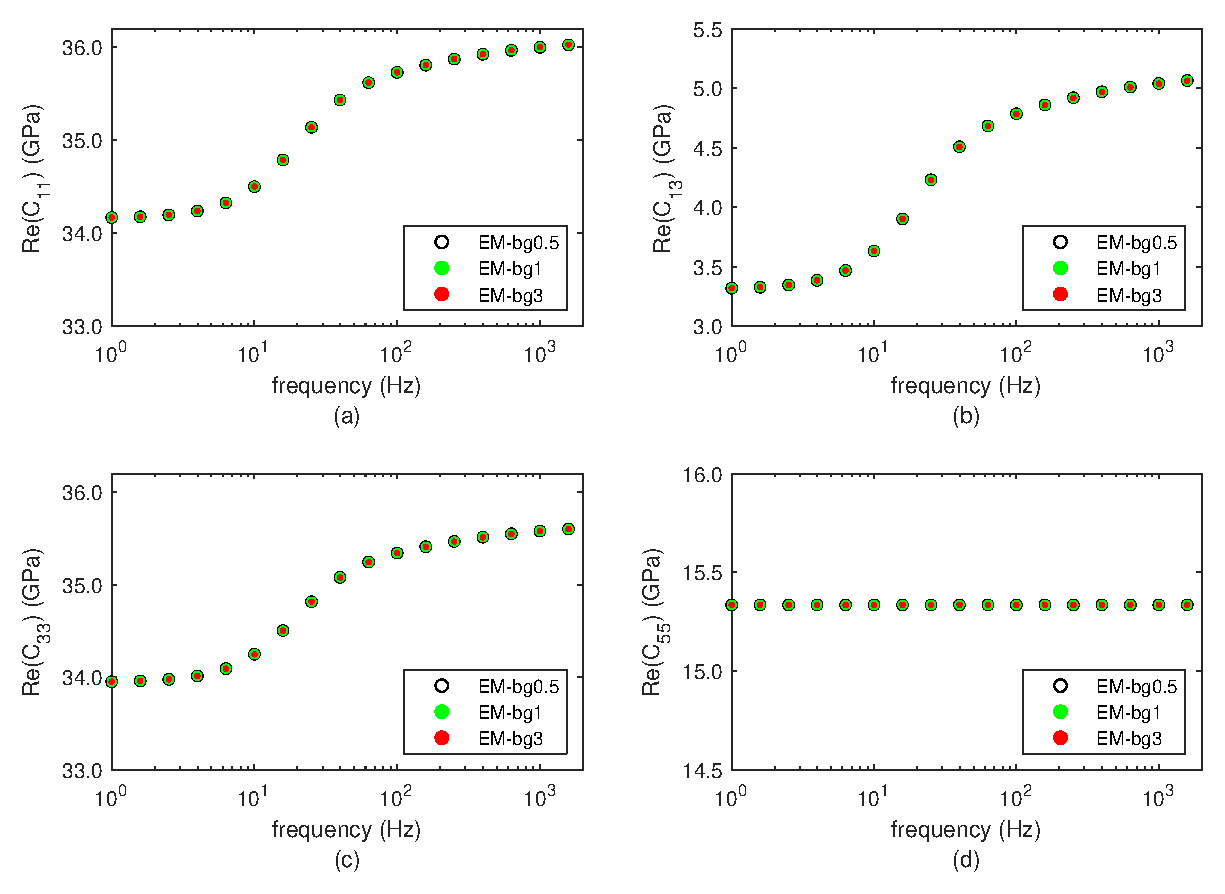
\includegraphics[width=100mm, height=80mm]{cijbg_2sandshale.eps}
\caption{Real part of the non-zero effective moduli as a function of frequency resulting from the homogenization of a thin layer consisting of a stack of two poroelastic sandstone beds, B1 and B2, embedded in elastic half-spaces. The moduli are obtained using three different samples $\Omega_e$ (Figure \ref{fig.1}) that consider background thicknesses that are half, one and three times the thickness of the thin layer. The corresponding curves are labeled EM-bg05, EM-bg1 and EM-bg3, respectively.}
\label{fig.2}
\end{figure}

%\begin{figure}[!ht]
%\centering
%        \includegraphics[width= 150mm, height=60mm]{maps_sandCombined.eps}
%\caption{Pressure maps for the vertical compressional oscillatory test at 39.8 Hz for homogenization procedures a) A that imposes a no-flow condition at top and bottom of the sample $\Omega$ and b) C that consider fully periodic BC on all boundaries of $\Omega$. See Figure \ref{fig.2}.}
%\label{fig.4}
%\end{figure}
Figure \ref{fig.3} shows plots of the real part of the non-zero effective moduli as a function of frequency obtained using samples that consider background thicknesses that are half, one and three times the thickness of the thin layer. The corresponding curves are labeled EM-bg05, EM-bg1 and EM-bg3, respectively. The results show that the estimated moduli are independent of the thickness of the sampled background, which implies that the only influence of the background is to affect the BC at the respective thin layer boundaries. 
On the other hand, we observe the homogenized medium is
characterized by vertical transverse isotropy (VTI) that results from the horizontal bedding of the two sandstones that constitute the thin layer. Therefore, the elements $C_{15}$ and $C_{35}$ of its stiffness matrix are zero. Notice as well that $\Re(C_{55})$  (Figure \ref{fig.3}d) is not frequency-dependent. This is because in VTI media, the shear relaxation oscillatory test, which is the analogous to a normal-incident S-wave, generates shear strains and stresses components  parallel to the bedding plane. However, such shear components are not locally perturbed by the fluid content of the beds since fluids cannot support shear stress. Moreover, this element reads $C_{55} = \langle \sigma_{13}\rangle\,/(\,2\, \langle \varepsilon_{13} \rangle\,)$ and it can be shown that this is equivalent to $C_{55}  =\left( \sum_i f_i/\mu_i \right)^{-1}$, where $f_i$ is the height fraction of the $i$th layer and $\mu_i$ is the corresponding shear modulus \cite{Backus1962, Salamon1968}. This value is 15.3 GPa for our example. The moduli  $C_{11}$, $C_{13}$ and $C_{33}$ are affected by FPD effects and therefore present a frequency dependent behavior. Specifically, the pressure gradient for FPD is controlled by the water-saturated region due to the lower compressibility compared to the gas-saturated counterpart. As a consequence, the deformation induced by the compressinal relaxation oscillatory tests creates  higher pressure increments in this region that equilibrate when the water diffuses into the gas-saturated pores of the adjacent sandstone bed. Similarly, the transition frequency of these moduli is controlled by the viscosity of water and thickness of the corresponding bed. Using Equations \eqref{Eq.3} and \eqref{Eq.5}, we find that this transition frequency is around 50.4 KHz. 

%Notice that both homogenization procedures reproduce this value (Figure \ref{fig.3}d). This shows that, given the VTI nature of the TPL, the estimation of this modulus is insensitive to the BC imposed at the TPL-background interface. However, this is not the case for the real part of elements $C_{11}$,  $C_{13}$ and $C_{33}$ where differences between the HTPL-bg and HTPL-p moduli are visible and in average they are around 1 GPa. In this regard, these discrepancies evidence the impact on the moduli estimations of the different BC incorporated in the homogenization procedures. For the proposed procedure, the presence of impermeable background in the sample induces a no-flow condition and a continuity of displacement and tractions at the boundaries of the TPL. In contrast, the traditional method imposes periodicity of these variables on analogous boundaries.

\begin{figure}[!ht]
\centering
        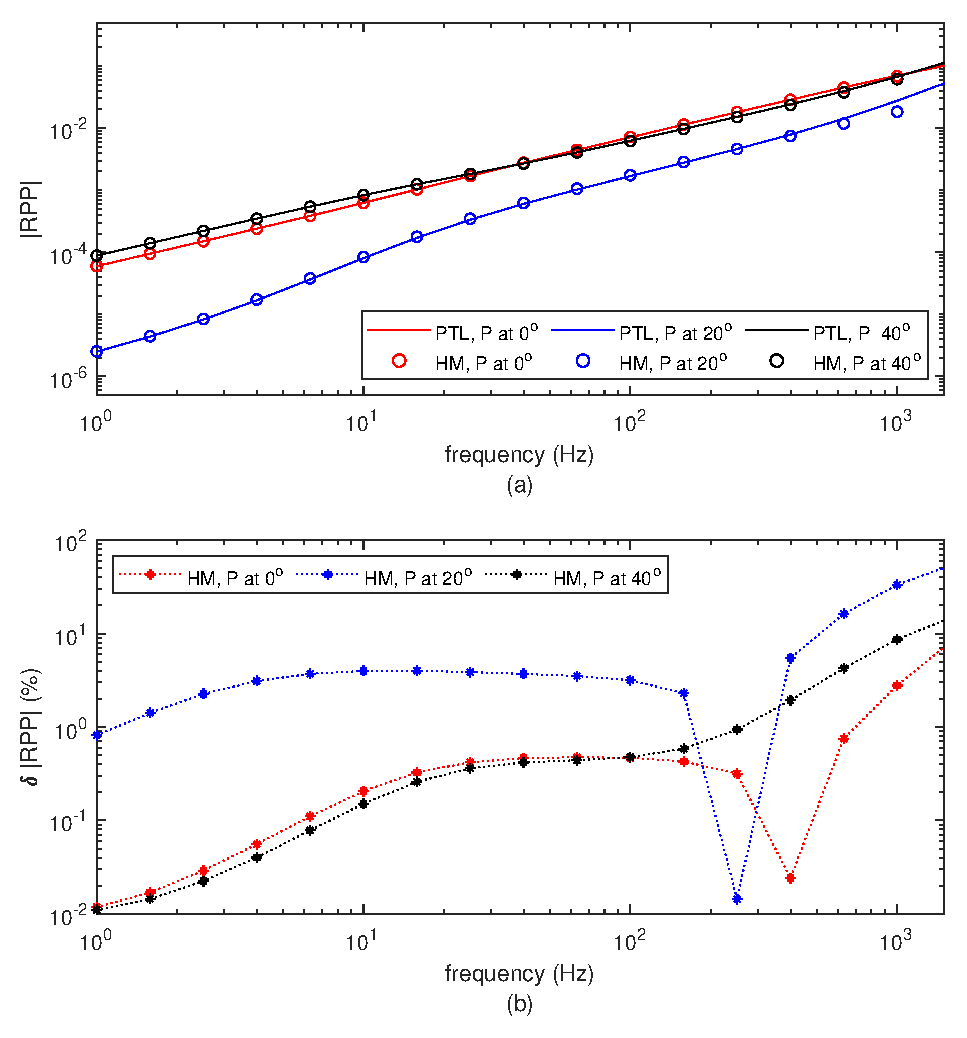
\includegraphics[width= 120mm, height=120mm]{rppbg_2sandshale.eps}
\caption{ (a) Absolute value of the PP reflection coefficients as a function of frequency for several angles of incidence calculated for the  model consisting of a thin layer comprised by two poroelastic sand beds embedded in elastic half-spaces and for the analogous model where the thin layer is replaced by the corresponding homogenized medium.  (b) Percentage errors of the absolute values of the PP reflection coefficients as a function of frequency calculated for the model using the homogenized medium. The acronyms PTL and HM of the curve labels stand for poroelastic thin layer and homogenized medium, respectively}
\label{fig.3}
\end{figure}

%\begin{figure}[!ht]
%\centering
%        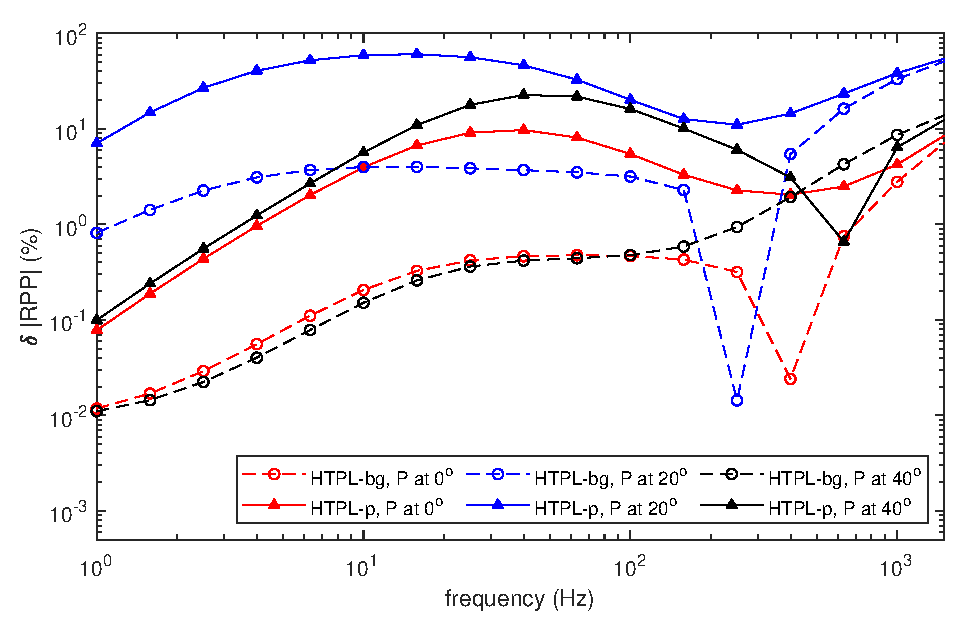
\includegraphics[width= 120mm, height=75mm]{rppdif_2sandshale.eps}
%\caption{Percentage errors of the absolute values of the PP reflection coefficients as a function of frequency calculated for the models using the HTPL-bg and HTPL-p, respectively
%for the same incident angles shown in Figure \ref{fig.4}.}
%\label{fig.5}
%\end{figure}

Next, we present the reflectivity results using the effective moduli as well as a comparison against the exact calculations. 
Figure \ref{fig.3}a shows the absolute value of the PP reflection coefficients with respect to frequency for three different angles of incidence calculated for the  thin layer model consisting of two poroelastic sand beds that is embedded in elastic half-spaces and for the analogous model where the poroelastic thin layer is replaced by its corresponding homogenized medium.  
Figure \ref{fig.3}b shows the percentage errors of the absolute value of the PP reflection coefficients as a function of frequency of the model using the homogenized medium for the same angles of incidence used in Figure \ref{fig.3}a. The acronyms PTL and HM shown in the curve labels stand for poroelastic thin layer and homogenized medium, respectively. 
These results show that the PP reflection coefficients obtained using the homogenized medium of the poroelastic thin layer reproduce, with acceptable errors, those obtained using the poroelastic thin model. In fact, for frequencies within the seismic range the errors are below 4\%, where maximum errors correspond to an incident angle of 20 degrees. On the other hand, the onset frequency at normal incidence of reverberations for the model using the homogenized medium is estimated to be around 9.7 KHz, which is out of the frequency of interest.
%In contrast,
%reflectivity deviations using using the HTPL-p are larger. The errors have a maximum of 60.5\% for an incident angle of 20 degrees and, in average, errors are consistently higher compared to the ones obtained using the HTPL-bg, presenting a maximum of 9.7\%  and 22.7\% for incident angles of 0 and 40 degrees, respectively.
%***********************
\section{Discussion}

\subsection{Effect of disregarding the background in the sample}

\begin{figure}[!ht]
\centering
        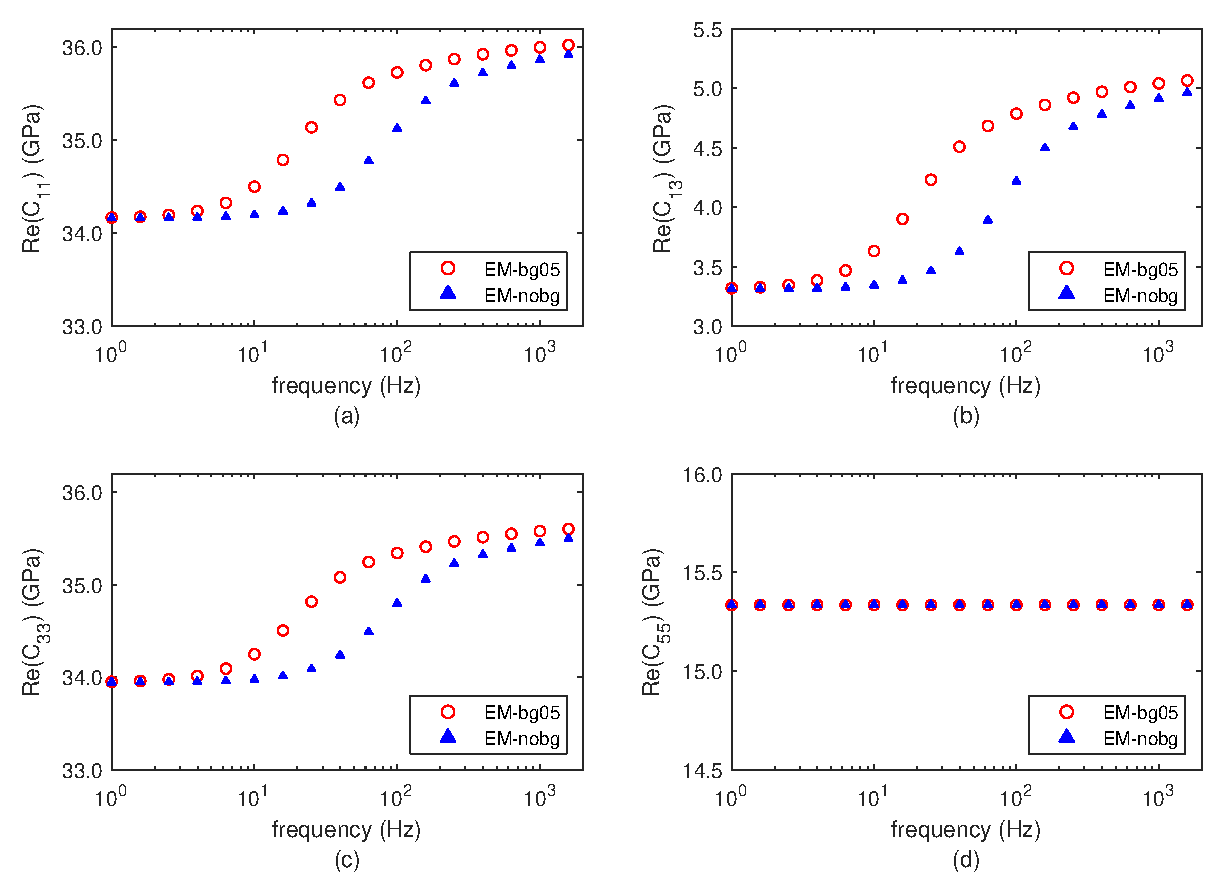
\includegraphics[width= 120mm, height=80mm]{cijbgcompare_2sandshale.eps}
\caption{Real part of the non-zero effective moduli as a function of frequency obtained after the homogenization of the poroelastic thin layer considered in the Results section using  both a sample that disregards the background (EM-nobg) and a sample that includes it (EM-bg05). This latter sample refers to the one used in the proposed homogenization procedure}
\label{fig.4}
\end{figure}

\begin{figure}[!ht]
\centering
        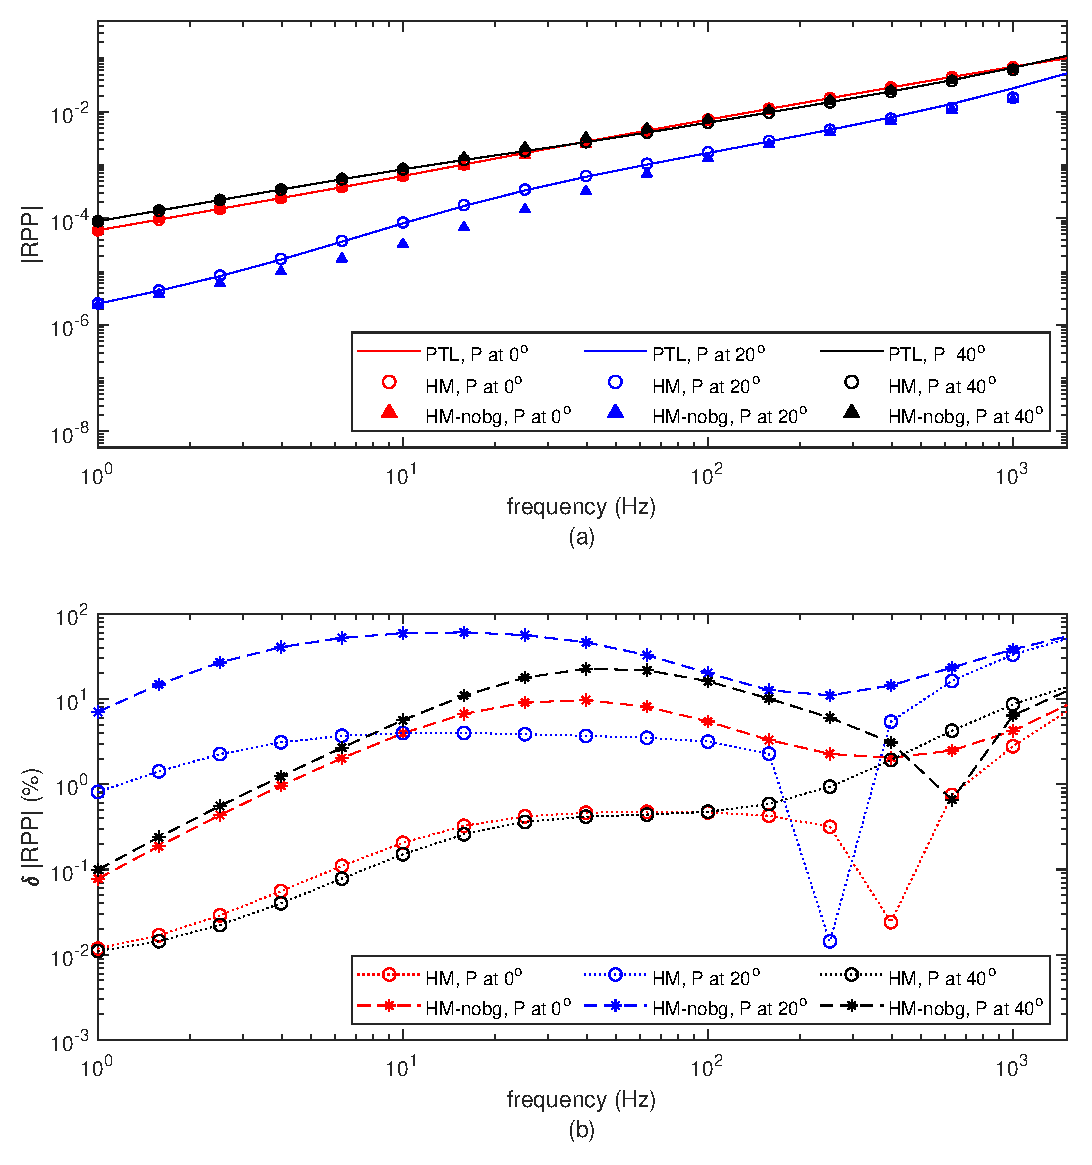
\includegraphics[width= 120mm, height=120mm]{rppbgcompare_2sandshale.eps}
\caption{a).Absolute value of PP reflection coefficients as a function of frequency for three angles of incidence calculated for the model that uses the poroelastic thin layer model described in the Results section (the cruves labels include the acronym PTL) and the analogous models that use the homogenized media obtained with samples that considers and disregard the background, respectively. The corresponding curves labels include the acronym HM and HM-nobg, respectively. b) Percentae errors of the absolute values of the PP reflection coefficients as a function of frequency calculated for the same angles of incidence and homogenized media considered in part (a).} 
\label{fig.5}
\end{figure}

We use the thin poroelastic layer considered in the previous section to investigate the impact of disregarding the background on the estimation of the effective moduli and, the effect that using this moduli has on the accuracy of the reflectivities computation compared to the ones obtained using the poroelastic thin layer. To this end, we take a sample that consists only of a representative section of the poroelastic thin layer $\Omega_p$ (Figure \ref{fig.1}b) to apply the homogenization procedure described in the Methodology section. However, for this case, the governing equations and oscillatory tests are used only over $\Omega_p$. We remark that this homogenization procedure applies periodic BC on the boundaries of $\Omega_p$, which is equivalent to regarding the sample as periodic.
Figure \ref{fig.4} shows the real part of the non-zero effective moduli as a function of frequency obtained using the sample $\Omega_p$ that disregards the background (curves labeled EM-nobg). For comparison we also have included the previously estimated moduli (curves labeled EM-bg05) obtained using the sample $\Omega_e$  that includes part of the background as detailed in the previous section. Results show that for the real part of the elements $C_{11}$, $C_{13}$ and $C_{13}$ there is a visible difference, that reaches a maximum values of around 1 GPa, between the curves obtained using the sample that disregards the background and the one that considers it. These discrepancies evidence the impact of the different BC incorporated in the homogenization procedures due to the sampling strategy. For the proposed method, the presence of the impermeable background in the sample induces a no-flow condition and a continuity  of displacement and tractions at the pertinent boundaries of the thin layer. In contrast, the homogenization procedure that disregards the background in the sample, imposes periodicity of these variables on analogous boundaries. On the other hand, as previously detailed, $C_{55}$ is not frequency dependent due to the VTI nature of the considered poroelastic thin layer. As previously explained, this moduli is unaffected by fluid effects and its closed form computation yields a value of 15.3 Gpa that, in this case, both homogenization procedures reproduce. This reveals that this modulus is insensitive to the BC imposed at the poroelastic thin layer-background interface.

Next, we compare the reflectivity results. Figure \ref{fig.5}a shows the  absolute values of the PP reflection coefficients as a function of frequency for three different angles of incidence calculated for the poroelastic thin layer embedded in half-spaces (curves beginning with the acronym PTL) and for the analogous models where the poroelastic thin layer is replaced by the corresponding homogenized media obtained with the samples that include and disregard the background, respectively (curves beginning with the acronym HM and HM-nobg, respectively). Figure \ref{fig.5}b shows the percentage errors of the absolute value of PP reflection coefficients as a function of frequency for the same angles of incidence and homogenized media considered in Figure \ref{fig.5}a.  As previously stated, the model that uses the homogenized medium obtained considering part of the background in the sample (proposed method) reproduces with acceptable errors, below 4\%, the reflectivities  within the seismic frequency range of the poroelastic thin layer. In contrast, reflectivity deviations using the homogenized medium obtained disregarding the background in the sample are larger. These errors rise up to a maximum of 60.5\% for an incident angle of 20 degrees and, in average, they are consistently higher compared to the ones obtained using the proposed homogenization method.

\subsection{Analysis of the boundary conditions induced by the impermeable background} 
In the previous subsection, we have stated that the background induces at the interfaces with the thin poroelastic layer a no-flow condition that results from its impermeable character and a continuity of displacement and tractions. Here, we investigate the extent to which such no-flow condition influences the estimation of the effective moduli. To this end, we  take a sample $\Omega_p$ (Figure \ref{fig.1}b) that consists only of a representative section  of the poroelastic thin layer considered in the Results section. Then, to incorporate the no-flow condition imposed by the background, we formulate such BC on the relevant boundaries of the sample $\Omega_p$ as part of the  oscillatory relaxation tests. To achieve this, we replace Equation \ref{Eq.11} by the following one
\begin{linenomath*}
\begin{equation}\label{Eq.14}
\begin{split}
& \nabla p \cdot \bm{\hat n}  = 0 \quad \text{on}\quad \Gamma_3^+ \, \cup \, \Gamma_3^+,\\
& p\vert_{\Gamma_1^+}-p\vert_{\Gamma_1^-} =0, \\
& \left(\bm{\sigma}\cdot \bm{\hat n} \right)\, \vert_{\Gamma_k^+}-\left(\bm{\sigma}\cdot \bm{\hat n} \right)\, \vert_{\Gamma_k^-} = \bm{0},\\
&\left( \frac{\kappa}{\eta} \nabla p \cdot \bm{\hat n} \right) \, \vert_{\Gamma_1^+} -\left( \frac{\kappa}{\eta} \nabla p \cdot \bm{\hat n} \right) \, \vert_{\Gamma_1^-} = 0.
\end{split}
\end{equation}
\end{linenomath*}
The first line of Equation \eqref{Eq.14} formulates the no-flow condition on the top and bottom boundaries of the sample $\Omega_p$. Notice that for this homogenization procedure, we still consider periodic BC for displacements. 

Figure \ref{fig.6} compares the real part of the effective moduli obtained with the homogenization procedure that applies the no-flow BC on the pertinent boundaries of a sample  $\Omega_p$ (curves labeled EM-nf) against those obtained after applying the proposed method that uses a sample that includes part of the embedding background (curves labeled EM-bg05). These results show that both procedures yield the same moduli. This further implies that to homogenize a poroelastic thin layer comprised of a stack of homogenous and isotropic beds, it is sufficient to account for the no-flow condition on the relevant boundaries of a sample $\Omega_p$. This outcome also suggests that, for this type of poroelastic thin layers, BC regarding displacements and tractions are not relevant for the estimation of the corresponding moduli. This is likely to be a consequence of the uniform stress-strain distribution along the background-thin layer interfaces resulting from the homogeneous character of the beds composing the thin layer.

\begin{figure}[!ht]
\centering
        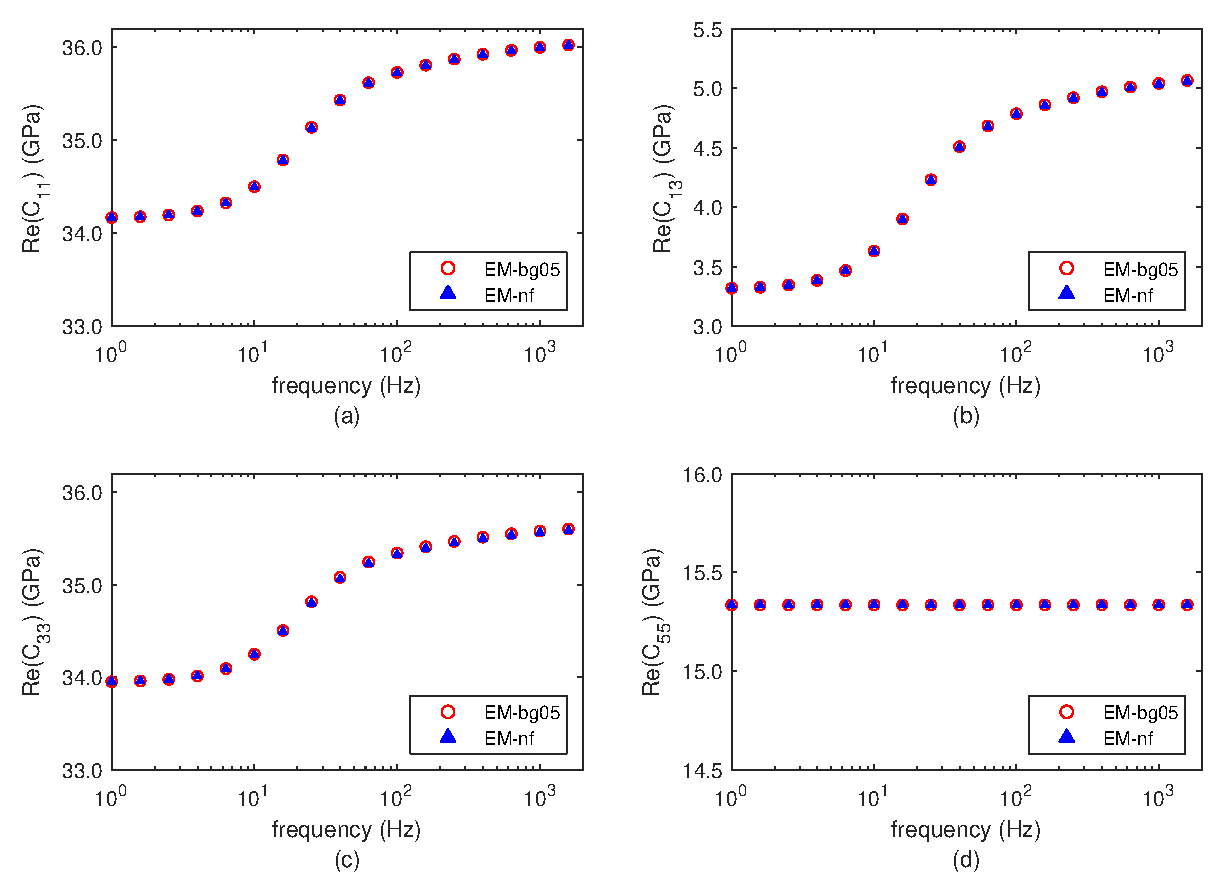
\includegraphics[width= 120mm, height=80mm]{cijnf_2sandshale.eps}
\caption{Real part of the non-zero effective moduli as a function of frequency obtained after applying the proposed homogenization method (curves labeled EM-bg05) and the homogenization procedure that uses a sample that disregards the background and applies no-flow BC on the relevant boundaries to emulate the impermeable character of the background (curves labeled EM-nf).}. 
\label{fig.6}
\end{figure}

Next, we test whether stress-strain concentrations at the boundaries of a poroelastic thin layer with the embedding background are likely to effect the estimated effective moduli. To this end, we consider a modified version of thin layer model used in the Results section as shown in Figure \ref{fig.7}. This new model incorporates inclusions with banded shapes that consist of a softer and less permeable material. These inclusions are located in the gas-saturated region, and they have one of their tips terminating at the thin layer upper boundary. They present the following physical properties: $K_m$ = 0.4 GPa,  $\mu$ = 0.2 GPa, $\kappa$ = $10^{-8}$ D, $K_s$ = 37 GPa, $\rho_s$ = 2700 g/kg$^3$ and $\phi$ = 0.05. Fluid properties correspond to those of water in Table \ref{table.2}. We homogenize this modified poroelastic thin layer applying both the homogenization procedure that formulates the no-flow BC on the pertinent boundaries of a sample $\Omega_p$ that disregards the background and the proposed homogenization procedure that use a sample $\Omega_e$ that incorporates a portion of the background. (Figure\ref{fig.7}).

\begin{figure}[!ht]
\centering
        \includegraphics[width= 80mm, height=70mm]{TPLgas_water_sand_bands.eps}
\caption{Poroelastic thin layer embedded in impermeable half-spaces $\Lambda_1$ and $\Lambda_2$. This model consists of the same sand layers B1 and B2 considered in the Results section. However, the upper sand presents inclusions with banded shapes with one of their tips terminating at upper boundary of the thin layer. The light blue boxes represent the samples $\Omega_e$ and $\Omega_p$ used for applying the proposed homogenization and the one that imposes a no-flow BC on the relevant boundaries to emulate the impermeability of the background, respectively.}. 
\label{fig.7}
\end{figure}

\begin{figure}[!ht]
\centering
        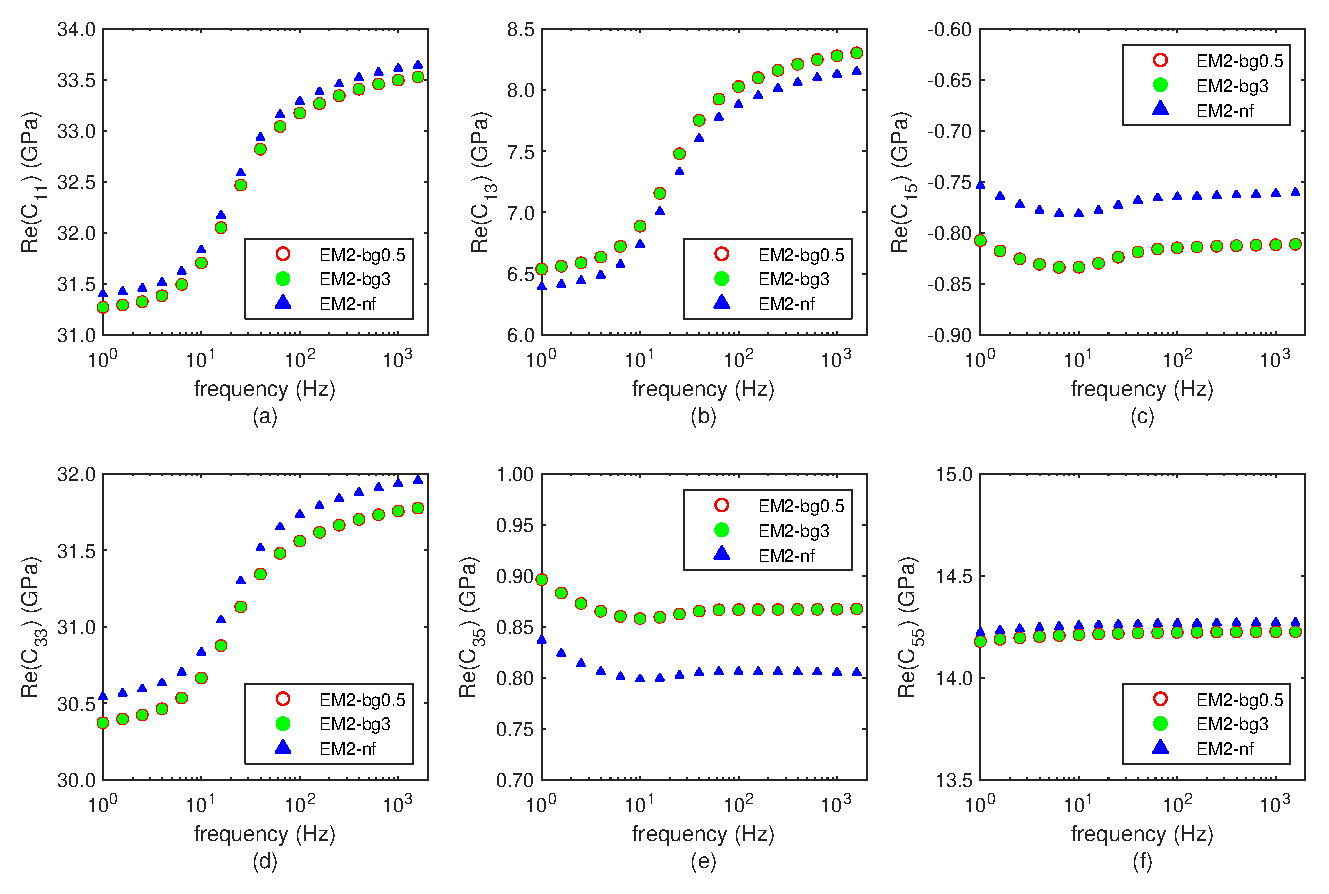
\includegraphics[width= 120mm, height=80mm]{cij_2sandfracw.eps}
\caption{Real part of the effective moduli as a function of frequency obtained after applying two different homogenization methods. One of them is the proposed homogenization procedure performed on samples $\Omega_e$ (Figure \ref{fig.7}) that consider background thicknesses that are half and three times the thickness of the thin layer (curves labeled EM2-bg05 and EM2-bg3, repectively) and the other one is the one that imposes no-flow BC on the relevant boundaries of the sample $\Omega_p$ (Figure \ref{fig.7}) (curves labeled EM2-nf). }. 

\label{fig.8}
\end{figure}

\begin{figure}[!ht]
\centering
        \includegraphics[width= 140mm, height=130mm]{strain_stress_sandfracw.eps}
\caption{Maps of the real part of the vertical stress component obtained for the thin layer samples a) $\Omega_e$  and b) $\Omega$ (Figure \ref{fig.7}). Maps of the real part of the vertical strain  obtained for the same samples c) $\Omega_e$  and d) $\Omega$. 
The sample $\Omega_e$ incorporates background with a thickness that is half of the thickness of thin layer.
The maps are obtained after applying the vertical compressional oscillatory test for a frequency of 39.8 HZ.}
\label{fig.9}
\end{figure}

\begin{figure}[!ht]
\centering
        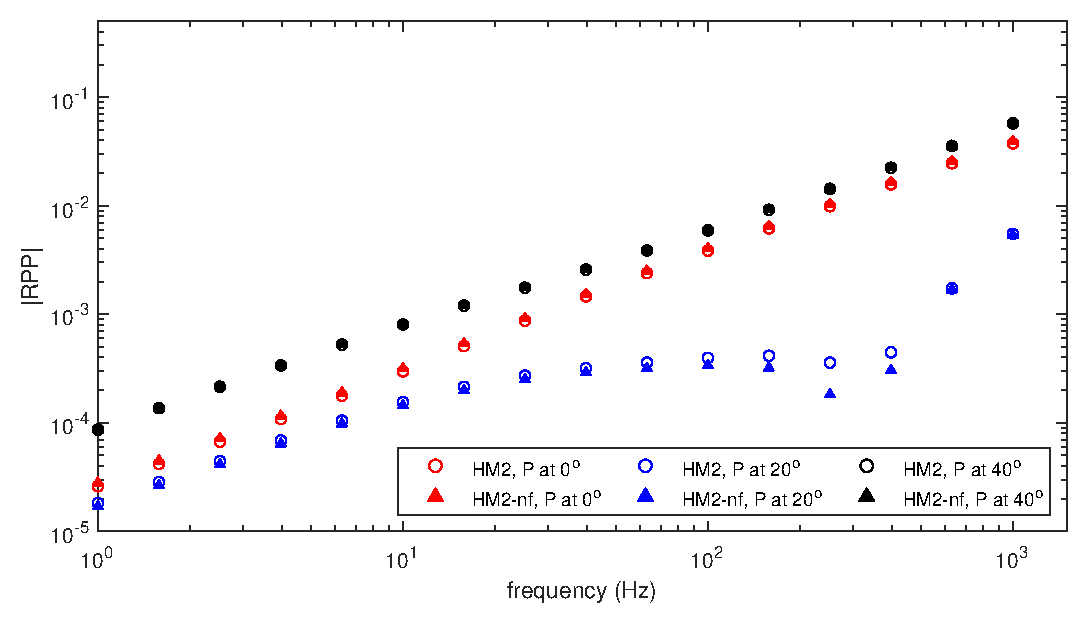
\includegraphics[width= 120mm, height=60mm]{rpp_2sandfracw.eps}
\caption{Absolute value of the PP reflection coefficients as a function of frequency for several angles of incidence calculated for the models using the homogenized medium obtained after applying the proposed homogenization procedure on the sample $\Omega_e$ (curves that include the acronym HM2) and the one that uses the sample $\Omega_p$ and imposes no-flow BC on the relevant boundaries (curves that include the acronym HM2-nf).}
\label{fig.10}
\end{figure}

Figure \ref{fig.8} shows the real part of the estimated effective moduli as a function of frequency obtained after applying the two aforementioned homogenization procedures.
The curves labeled EM2-bg05 and EM2-bg3 refer to the moduli obtained using samples $\Omega_e$ that consider background thicknesses that are half and three time the background of the modified thin layer model and the curve labeled EM2-nf refers to the moduli obtained using the homogenization procedure that formulates the no-flow BC on the relevant boundaries of the sample $\Omega_p$. The results show that the moduli obtained using the proposed method are independent of the size of the sampled background. On the other hand, there is a visible difference between the moduli obtained applying the two homogenization procedures.% homogenization procedure that formulates the no-flow BC on the relevant boundaries of the sample $\Omega_p$ and the proposed homogenization procedure that considers part of the embedding background in the sample. 
 This disagreement is likely related to differences in the regions affected by the stress-strain concentrations. To further investigate this aspect, we compare the corresponding stress and strain maps obtained after applying the vertical compressional relaxation test for a frequency of 39.8 HZ. Figures \ref{fig.9}a and \ref{fig.9}b show maps of the real part of the vertical stress components obtained on a sample $\Omega_e$ that includes background with half of the thickness of the considered thin layer and on a sample $\Omega_p$ that disregards the background, respectively. Similarly, Figures
 \ref{fig.9}c and \ref{fig.9}d show maps of the real part of the vertical strain components obtained on the same samples  $\Omega_e$ and $\Omega_p$, respectively under the same oscillatory test. Notice that in both cases, the vertical compressional test creates stress-strain concentrations in the vicinity of the tips of the inclusions. However, the regions affected around the the upper edges of the inclusion are different for the different samples. For the sample $\Omega_e$, this stress-strain concentration affects a region outside the thin layer section that includes a section of the  background in the vicinity of the upper boundary of the thin layer (Figures \ref{fig.9}a and \ref{fig.9}c). In contrast, for the sample $\Omega_p$  the corresponding stress-strain concentrations affect a region inside the thin layer section in the vicinity of its bottom boundary as a consequence of the periodic character of the BC for displacements and tractions (Figure \ref{fig.9}b and \ref{fig.9}d). This shows that the homogenization procedure that formulates the no-flow BC on the relevant boundaries of $\Omega_p$ considers an additional region of stress-strain concentration at the bottom boundary of the thin layer section when performing the averaging of these components. Hence, applying the proposed homogenization methodology is likely to reproduce more closely the actual stress-strain concentrations since they affect only the regions in the vicinity of the edges of the inclusions, which in this case, includes a part of the background close to the thin layer upper boundary as shown in Figures \ref{fig.9}a and \ref{fig.9}c. On the other hand, for the reflectivity calculations, we can still assume that the upper half-space behaves as an homogeneous material despite of the region affected by the strain-stress concentrations because this region is in general much smaller than the considered wavelength.

To compare the effect that the corresponding estimated moduli have on  reflectivity, we present the respevitve results in Figure \ref{fig.10}. This figure shows the absolute values of PP reflectivities as a function of frequency for several angles of incidence calculated for the model that uses the homogenized medium obtained applying the proposed homogenization procedure (curves including the acronym HM2) and for the model that uses the homogenized medium resulting from applying the procedure that incorporates the no-flow BC on the relevant boundaries of a sample $\Omega_p$ (curves including the acronym HM2-nf). Notice that some discrepancies are visible, specially for an incident angle of 20 degrees. Although there is no analytical solution available for the corresponding poroelastic thin layer model, it is likely that the model using the homogenized medium obtained after applying the proposed homogenization method reproduces more closely the actual reflectivities for the reasons previously argued. %Nonetheless, numerical computations of reflectivities of complex TPL models is a pending subject for future research.

%Although, computations of the TPL2 reflectivities can be performed applying numerical methods, we consider that th
In this subsection, we have shown that for the homogenization of poroelastic thin layer models consisting of a stack of few homogeneous beds and that are embedding in impermeable background, it is sufficient to impose the no-flow BC on the relevant boundaries of a sample that takes only a representative section of the thin layer to find a good estimation of the corresponding effective viscoelastic moduli. Nevertheless, this is no longer the case for poroelastic thin layer models that consider more complex geometries which can create stress-strain concentrations at the thin layer boundaries. For these latter cases, evidence suggests that the proposed homogenization methodology reproduces more reasonably the expected regions of  stress-strain concentrations and therefore it is likely to yield better estimates of the corresponding effective moduli.

\subsection{Effect of the background permeability}

\begin{figure}[!ht]
\centering
        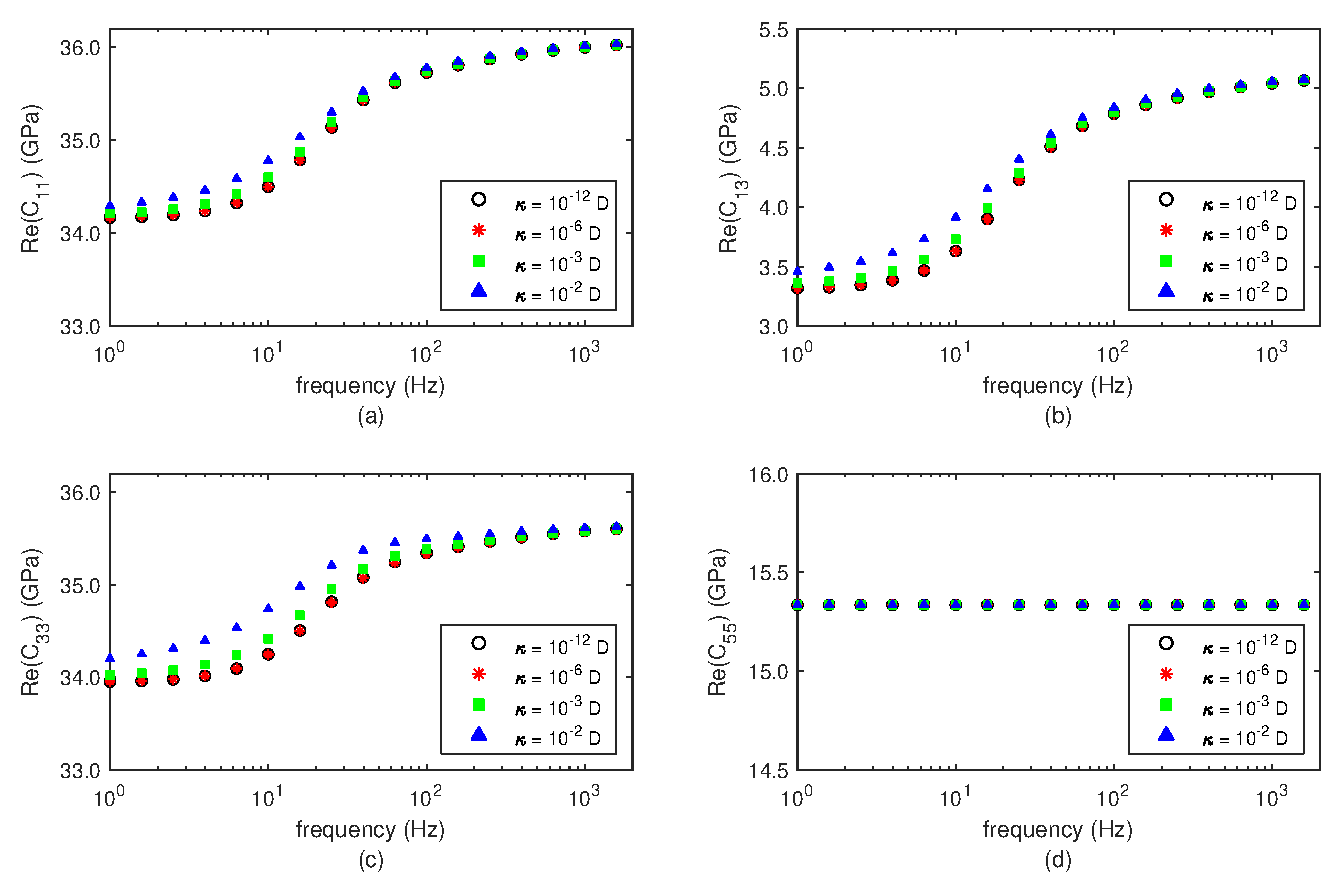
\includegraphics[width= 120mm, height=80mm]{cijkbg_2sandshale.eps}
\caption{Real part of the non-zero effective moduli as a function of frequency obtained after applying the proposed homogenization method to samples $\Omega_e$ of the poroelastic thin layer considered in the Results section. The samples include background with different permeabilities $\kappa$.}
\label{fig.11}
\end{figure}

\begin{figure}[!ht]
\centering
        \includegraphics[width= 120mm, height=140mm]{pressure_kbg.eps}
\caption{Maps of the real part of the pressure obtained after applying the vertical compressional oscillatory test at 10 Hz to samples $\Omega_e$ of the thin layer model used in the Results section. This samples include background with a thickness that is half of the thickness of the thin layer and with permeabilities $\kappa$ equal to a)$10^{-12}$ D, b)$10^{-6}$ D, c)$10^{-3}$ D and d)$10^{-2}$ D. }
\label{fig.12}
\end{figure}

For this study we have assumed that the background embedding the poroelastic thin layer is impermeable for the frequencies of interest. This assumption ensures that FPD effects and, therefore, the induced effective dispersive behavior of P-and S-waves are confined within the thin layer. This feature is particular amenable for finding the corresponding effective viscoelastic equivalent capable of reproducing the reflectivity response of the poroelastic thin layer, as it has been shown in the current study. On the other hand, considering an impermeable background renders the modeling computational efficient since it allows using the elastic framework. Nonetheless, the pending question is regarding an appropriate permeability threshold of the embedding background that can still warrant that the aforementioned assumptions are met for the seismic frequencies of interest. Thus, in the following, we investigate up to which extent the permeability of the background can be decreased in such a way that it can be still considered impermeable for the seismic frequency range.
% Meaning that, for such permeabilities, FPD effects induced at the background-thin layer interfaces are not relevant for the frequency range considered.
To this end, we consider the same thin layer model as used in the Results section. However, for this case we assume that the permeability of the embedding background takes the lower values of $10^{-6}$ D, $10^{-3}$ D and $10^{-2}$ D, respectively than the previously assigned ($10^{-12}$ D, Table \ref{table.1}). Then, we apply the proposed homogenization procedure to samples that consider a background thickness that is half of the thin layer thickness. 

Figure \ref{fig.11} shows the real part of the non-zero effective moduli as a function of frequency obtained after applying the proposed homogenization method to samples that consider background with different permeabilities $\kappa$. For comparison, we also present the moduli obtained with the same background permeability of $10^{-12}$ D considered in the Results section.
Results show that the moduli obtained with the two lowest background permeabilities of $10^{-12}$ D and $10^{-6}$ D overlay for practical purposes, indicating that the assumption of an impermeable background holds for these permeabilities for the considered frequencies. In contrast, there are increasingly visible differences, with respect to the reference moduli, ($\kappa = 10^{-12}$ D for those moduli obtained using background permeabilities that take the lower values of  $10^{-3}$ D  and $10^{-2}$ D, respectively, revealing that FPD effects between the background and poroelastic thin layer interfaces become progressively stronger. This is specially evident for frequencies below 100 Hz, in which the relaxed and the transition FPD regimes prevail. To further investigate the effect of the background permeability on FPD effects with the adjacent poroelastic thin layer, we analyze the maps of the real part of the pressure (Figure \ref{fig.12}) obtained after applying the vertical compression test at 10 Hz to samples that include background with the permeabilities shown in Figure \ref{fig.11}.
Notice that the maps corresponding to the background permeabilities of $10^{-12}$ D (Figure \ref{fig.11}a) and $10^{-6}$ D (Figure \ref{fig.11}b) show an abrupt jump of pressure at the background-thin layer interfaces. This is the outcome of the impermeable character of the background that isolates the hydraulic communication with the thin layer. 
However, as the background permeability takes the lower values of $10^{-3}$ D (Figure \ref{fig.11}d) and $10^{-2}$ D (Figure \ref{fig.11}e), respectively, the pressure change at the interfaces becomes progressively less sharp. Indeed, the maps show an increasingly larger pressure transition zone that takes place at the background side of the background-thin layer interfaces as the background permeability increases. 
This pressure transition zone is a consequence of FPD occurring between the background and the thin layer as a result of the hydraulic communication between them. In this case, the fluid flows from the more pressurized background towards the less pressurized thin layer producing the decrease of pressure observed at the background side of the corresponding interfaces. On the other hand, this background-thin layer FPD effect implies that the proposed homogenization procedure is not directly applicable because we can no longer assume that a viscoelastic behavior is confined within the thin layer region since, in reality, this viscoelastic character extends beyond the thin layer boundaries due to such FPD effect. However, background rocks of interest such as shale and crystalline rocks in their intact state can exhibit permeabilities in the range of nano ( $10^{-6}$) to micro ($10^{-9}$) Darcies  \cite<e.g.,>{Mitchell2012, Fisher2017, Wenning2018, Zhao2018} which, as suggested by the current analysis, can be considered as impermeable for the seismic frequencies.


%\begin{figure}[!ht]
%\centering
%        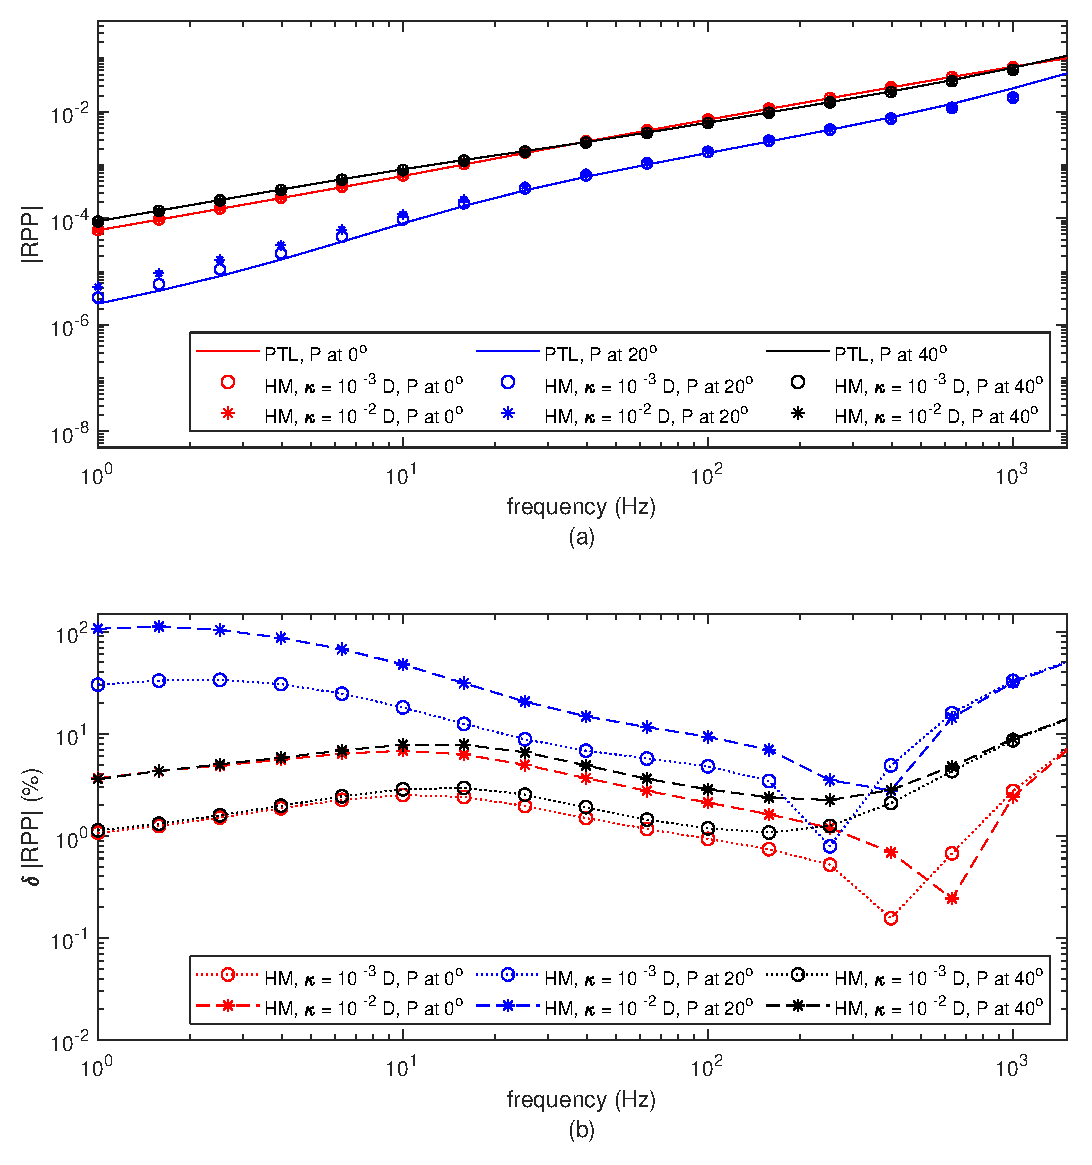
\includegraphics[width= 120mm, height=120mm]{rppkbg_2sandshale.eps}
%\caption{ (a) Absolute value of the PP reflection coefficients as a function of frequency for several angles of incidence calculated   (b) Percentage errors of the absolute values of the PP reflection coefficients as a function of frequency calculated y}
%\label{fig.13}
%\end{figure}


\section{Conclusions}
We have proposed a homogenization approach that incorporates the appropriate BC to estimate the effective moduli of thin layers embedded in impermeable background and that are composed of a stack of few poroelastic beds with distinct fluid and rock properties. This is accomplished by first, taking a sample that incorporates a portion of the background and a representative section of the thin layer and second, by performing the averaging of stress and strain components only over the thin layer section of interest.
The results show that the proposed methodology yields effective moduli capable to closely reproduce the reflectivity of such thin layers. In contrast, the effective moduli obtained under the traditional consideration of periodicity renders reflectivity results with larger errors. We  have also shown that for thin layers presenting beds with homogeneous properties, it is possible to disregard the background in the sample and replace its influence by a no-flow BC. However, this is no longer the case for thin layers that present heterogeneities with sharp edges close to their boundaries since they induce stress-strain concentrations that cannot be accounted by just imposing a no-flow BC. For such cases, our study suggests that the proposed homogenization procedure yields more reasonable estimates of the effective moduli, which implies that this methodology can be applied to strongly heterogenous poroelastic thin layers. On the other hand, our study also suggests that to ensure the validity of the proposed homogenization method, the background must behave as impermeable for the frequencies of interest. Otherwise additional background-thin layer FPD effects can enlarge the viscoelastic region beyond the thin layer boundaries. However, it is very likely that common background rocks with permeabilities in the $\mu$D order and lower comply with this requirement.



% Appendix
%*****************
\appendix
\section{PP reflectivity  at an elastic-poroelastic interface}

\subsection{Governing equations}
We consider a model in $\mathbb R^2$ consisting of 
$m$-poroelastic layers  $\Omega_{p1}$,  $\Omega_{p2}$,\dots, $\Omega_{pm}$ that are embedded in elastic half-spaces $\Lambda_1$ and $\Lambda_2$. Furthermore, we denote as $\Pi_1$  the interface between the upper half-space $\Lambda_1$ and the uppermost poroelastic layer $\Omega_{p1}$ and as $\Pi_{(m+1)}$ the interface between the lowermost poroelastic layer $\Omega_{pm}$ and the lower elastic half-space $\Lambda_2$. To compute the  reflection coefficients, we formulate the corresponding poroelastic and elastic wave equations in the space-frequency domain. To specify the poroelastic wave equation,  we let $\bm{u}^p =\bm{u}^p( \bm{x}, \omega)$ and $\bm{w} =\bm{w}( \bm{x}, \omega)$  be the solid displacement vector and the relative fluid displacement vector, respectively for any position $\bm{x} \in z$ with $z=\{\Omega_{p1},\dots,\Omega_{pm}\}$  and angular frequency $\omega \in I$, with $I =(0,W]$. Moreover, we let $\bm {\sigma}^p$, be the total stress which acts upon the PM. Then, we express the corresponding equation of motion as
\begin{linenomath*}
\begin{equation}\label{Eq.a1}
\begin{split}
& -\,\omega^2  \, \rho_b  \, \bm{u}^p -  \,\omega^2 \, \rho_f \, \bm{w}= \nabla . \, \bm{\sigma}^p \quad  \textrm{in} \quad z \times I, \\
& -\,\omega^2  \, \rho_f \, \bm{u}^p - \omega^2 g(\omega) \, \, \bm{w} + i \, \omega \, b(\omega) \, \bm{w} = - \nabla \, p_f \quad  \textrm{in} \quad z \times I.
\end{split}
\end{equation}
\end{linenomath*}
The constitutive equations are
\begin{linenomath*}
\begin{equation}\label{Eq.a2}
\begin{split}
& \bm{\sigma}^p = \mu \,  \left( \nabla \,\bm{u}^p + ({\nabla  \bm{u}^p})^T  \right) +  \left( \lambda \, \nabla . \, \bm{u}^p\, + \alpha \,M \, \nabla . \, \bm{w} \right) \bm{I}, \\
&p_f=- \alpha \, M \, \nabla . \, \bm{u}^p - M \, \nabla . \, \bm{w},  \end{split}
\end{equation}
\end{linenomath*}
where $\rho_b$ and $\rho_f$ are the bulk density of the saturated porous medium and the density of the pore fluid, respectively,  $\lambda$ is the undrained Lamé modulus, and $g(\omega)$ and $b(\omega)$ are the mass coupling and viscous coefficients, respectively. The required material properties are calculated as follows \cite<e.g.,>{Barbosa2016}
\begin{linenomath*}
\begin{equation}\label{Eq.a3}
\begin{split}
& \rho_b =(1-\phi)\rho_s + \phi \rho_f, \\
& \lambda= K_m - \frac{2}{3} \mu + \alpha^2 M, \\
& g(\omega) =  \frac{1}{\omega} \Im \left( \frac{\eta}{\kappa_d(\omega)} \right),\\
& b(\omega) = \Re\left( \frac{\eta}{\kappa_d(\omega)} \right),
\end{split}
\end{equation}
\end{linenomath*}
where $\rho_s$ is the density of the solid grain and $\kappa_d(\omega)$ is the dynamic permeability of the porous rock, which can be expressed as \cite{Johnson1987}
\begin{linenomath*}
\begin{equation}\label{Eq.a4}
    \kappa_d(\omega)=\kappa \left(\sqrt{1 + \frac{4 i \omega}{n_j \omega_B} }+ \frac{i \omega}{\omega_B}   \right) ^{-1}.
\end{equation}
\end{linenomath*}
Here, $\omega_B$ is  Biot's angular characteristic frequency $\omega_B = 2 \pi f_B$, with $f_B$ defined in equation \ref{Eq.1}, and $n_j$ is a pore geometry parameter. According to numerical and experimental studies \cite<e.g.,>{Charlaix1988, Sheng1988, Smeulders1992}, $n_j$ = 8 is a reasonable approximation for most porous media.

To formulate the elastic wave equation, we let $\bm{u}^e=\bm{u}^e (\bm{x},\omega)$ be the displacement vector for any position $\bm{x} \in n$ with $n = \{\Lambda_1,\Lambda_2\}$  and angular frequency $\omega \in I$, with $I =(0,W]$. We also let $\bm{\sigma}^e$ be the stress tensor field acting upon the medium. Then, we express the corresponding equation of motion as
\begin{linenomath*}
\begin{equation}\label{Eq.a5}
- \, \rho_b \,\omega^2 \, \bm{u}^e = \nabla . \, \bm{\sigma}^e  \quad  \textrm{in} \quad n \times I.
\end{equation}
\end{linenomath*}
The associated constitutive equation is given by
\begin{linenomath*}
\begin{equation}\label{Eq.a6}
\bm{\sigma}^e = \mu \,  \left( \nabla \, \bm{u}^e + ({\nabla  \bm{u}^e})^T  \right) + \lambda \,  \nabla . \, \bm{u}^e\,\, \bm{I}.
\end{equation}
\end{linenomath*}
 
\subsection{Solution for displacements}
We assume that a P-wave propagates downwards, with wavevector components in $\bm{\hat x_1}$ and  $\bm{\hat x_3}$, and strikes the interface $\Pi_1$.  Then, in the elastic half spaces $n$, with $n =\{\Lambda_1,\Lambda_2\}$, the propagating modes  are P- and S-waves. In the poroelastic layers $z$, with $z=\{\Omega_{p1},\dots,\Omega_{pm}\}$, fast P-, slow P- and S-waves are present.

For a given poroelastic layer $z$, we write the total solid displacement $\bm{u}_z^p$  and relative fluid displacement $\bm{w}_z$ as
\begin{linenomath*}
\begin{equation}\label{Eq.a7}
\begin{split}
& \bm{u}_z^{p} =  \sum_r \bm{u}_{z\,r}^p, \\
& \bm{w}_z =  \sum_r \bm{w}_{z\,r},
\end{split}
\end{equation}
\end{linenomath*}
with $r=\{D_{P1},U_{P1},D_{P2},U_{P2},D_{S},U_{S}\}$. Here, $D$ and $U$ refer to the downgoing and upgoing waves, respectively, and subscripts $P1$, $P2$, and $S$ refer to fast P-, slow P- and S-waves, respectively,

For a given elastic-half space $n$,  we express the total displacement $\bm{u}_n^e$ as
\begin{linenomath*}
\begin{equation}\label{Eq.a8}
\bm{u}_n^{e} =  \sum_j \bm{u}_{n\,j}^e.
\end{equation}
\end{linenomath*}
Here, for $n =\Lambda_1 $,  $j=\{D_P,\,U_P,\,U_S\}$; otherwise, for $n =\Lambda_2 $, $j=\{D_P,\,D_S\}$. Subscripts $P$  and $S$ refer to P- and S-waves, respectively. 

We propose the solution for displacements in the form of scalar and vector potentials. Then, we express the displacements for the elastic half-spaces as
\begin{linenomath*}
\begin{equation}\label{Eq.a9}
\begin{aligned}
& \bm{u}_{n\,j_1}^e = \nabla \Phi^e_{n\,j_1},
\end{aligned}
\qquad
\begin{aligned}
& \bm{u}_{n\,j_2}^e = -  \nabla  \times \bm{\Psi}^e_{n\,j_2}.
\end{aligned}
\end{equation}
\end{linenomath*}
For $n =\Lambda_1 $,  $j_1 = \{U_P,\,D_P\}$,  while for $n =\Lambda_2 $, $j_1 = \{D_P\}$ and $j_2=j \setminus j_1$ for both cases. Moreover, $\Phi^e_{n\,j_1}$ and $\bm{\Psi}^e_{n\,j_2}$ are the scalar potentials corresponding to solutions for P-waves and the vector potential corresponding to solutions for S-waves, respectively. The potentials can be specified as
\begin{linenomath*}
\begin{equation}\label{Eq.a10}
\begin{split}
&  \Phi^e_{n\,j_1} = E_{n\,j_1} \exp \left( i\, \bm{k}_{n\, j_1}\cdot \bm{x} \right), \\
& \bm{\Psi}^e_{n\,j_2} =  E_{n\,j_2} \exp \left( i\, \bm{k}_{n\, j_2} \cdot \bm{x} \right) \bm{\hat {x}_2}, 
\end{split}
\end{equation}
\end{linenomath*}
where $E_{n\,j_1}$ and $E_{n\,j_2}$ are the amplitudes for the escalar and vector potentials, respectively and $\bm{k}_{n \,j_1}$, and $\bm{k}_{n\, j_2}$ are the wavenumber vectors for the P- and S-waves, respectively. The wavenumber vectors can be expressed as $\bm{k}_{n j} = k_{nj} \, \bm{\hat {k}_{nj}}$, where $\bm{\hat {k}_{n\, j}}$ is the unit wavenumber vector and $k_{n\,j}$ is the scalar wavenumber for the corresponding wave $j$. This latter depends only on the properties of the medium and on the wave type, that is, P or S. The scalar wavenumber can be written as
\begin{linenomath*}
\begin{equation}\label{Eq.a11}
\begin{split}
& k_{n\,j_1}  = \omega \sqrt{\frac{\rho_n}{\lambda_n + 2 \mu_n}}, \\[10pt]
& k_{n\,j_2}  = \omega \sqrt{\frac{\rho_n}{ \mu_n}}.
\end{split}
\end{equation}
\end{linenomath*}
%write P and S wavenumber equation%

For the poroelastic layers, we also express the solid and relative fluid displacements in term of potentials
\begin{linenomath*}
\begin{equation}\label{Eq.a12}
\begin{aligned}
& \bm{u}_{z\,r_1}^p = \nabla \Phi^p_{z\,r_1},
\end{aligned}
\qquad
\begin{aligned}
& \bm{u}_{z\,r_2}^p = - \nabla \times \bm{\Psi}^p_{z\,r_2},
\end{aligned}
\end{equation}
\end{linenomath*}
%*************
\begin{linenomath*}
\begin{equation}\label{Eq.a13}
\begin{aligned}
& \bm{w}_{z\,r_1} = \nabla \Theta_{z\,r_1},
\end{aligned}
\qquad
\begin{aligned}
& \bm{w}_{z\,r_2} = -  \nabla \times \bm{T}_{z\,r_2},
\end{aligned}
\end{equation}
\end{linenomath*}
where  $r_1 = \{D_{P1},\,U_{P1},\,D_{P2},\,U_{P2}\}$ and $r_2=r\setminus r_1$, 
$\Phi^p_{z\,r_1}$ and $\Theta_{z\,r_1}$ are the scalar potentials corresponding to solutions for P1- and P2-waves for the solid and the relative fluid displacements, respectively. Likewise $\bm{\Psi}^p_{z\,r_2}$ and $ \bm{T}_{z\,r_2}$ are the vector potentials corresponding to solutions for S-waves for the solid and the relative fluid displacements, respectively. The scalar and vector potentials can be further specified as
\begin{linenomath*}
\begin{equation}\label{Eq.a14}
\begin{split}
&  \Phi^p_{z\,r_1} = B_{z\,r_1} \exp \left( i\, \bm{k}_{z\, r_1}\cdot \bm{x} \right), \\
& \Theta_{z\,r_1} =  W_{z\,r_1} \exp \left( i\, \bm{k}_{z\, r_1} \cdot \bm{x} \right), 
\end{split}
\end{equation}
\end{linenomath*}
\begin{linenomath*}
\begin{equation}\label{Eq.a15}
\begin{split}
& \bm{ \Psi}^p_{z\,r_2} = B_{z\,r_2} \exp \left( i\, \bm{k}_{z\, r_2}\cdot \bm{x} \right) \bm{\hat {x}_2}, \\
& \bm{T}_{z\,r_2} =  W_{z\,r_2} \exp \left( i\, \bm{k}_{z\, r_2} \cdot \bm{x} \right) \bm{\hat {x}_2}, 
\end{split}
\end{equation}
\end{linenomath*}
where $B_{z\,r1}$ and $W_{z\,r1}$ are the amplitudes of the scalar potentials corresponding to the solid and relative fluid displacements, respectively. Likewise, $B_{z\,r2}$ and $W_{z\,r2}$, are the amplitudes of the vector potentials corresponding to the solid and relative fluid displacements, respectively. Moreover, $\bm{k}_{z\, r_1}$ is the complex wavenumber vector for P1- and P2-waves and $\bm{k}_{z\, r_2}$ is the one for S-waves. Besides,  the  presence of the enclosing elastic half-spaces induces inhomogeneous waves in the poroelastic layers. This is because Snell's law imposes the continuity of the horizontal component of the wavenumber vectors across the different media and the presence of the an elastic media enforces this component to be real. Thus, attenuation can only prevail in the vertical direction. Then, we can specify the complex wavenumber vector as
\begin{linenomath*}
\begin{equation}\label{Eq.a16}
\bm{k}_{zr}= \bm{\varkappa}_{zr} - i\, \bm{\alpha}_{zr},
\end{equation}
\end{linenomath*}
where $\bm{\alpha}_{zr}$ is the attenuation vector which has only a component in $\bm{\hat{x}_3}$ and $\bm{\varkappa}_{zr}$ is the real wavenumber vector. This latter can be expressed as $\bm{\varkappa}_{zr} = \varkappa_{zr} \bm{\hat{\varkappa}}_{zr}$, where $\varkappa_{zr}$ and $\bm{\hat{\varkappa}}_{zr}$  are the  real wavenumber and unit vector, respectively. For a given incidence angle striking at the interface between the upper half-space and the top most poroelastic layer, Snell's law states that the horizontal component of the real wavevector of the traveling waves are equal to that of the incident wave $p_i$. This is $p_i = \bm{k}_{nj} \cdot \bm{\hat{x}_1} =\bm{\varkappa}_{zr} \cdot \bm{\hat{x}_1} = \varkappa_{zr} \sin(\theta_{zr})$, where $\theta_{zr}$ is the angle of the real wave vector with respect to the vertical. 
We express the missing vertical component of the complex wavenumber vector as follows: $\bm{k}_{zr} \cdot \bm{\hat{x}_3}= \varkappa_{zr}\cos (\theta_{zr}) - i\, \alpha_{zr}$, where $\alpha_{zr}$
is the attenuation factor. Following \citeA{Borcherdt1982} we find
\begin{linenomath*}
\begin{equation}\label{Eq.a17}
\begin{split}
& \varkappa_{zr}^2 =p_i^2 + \left(\Re\,[\left( k_{zr}^2 -  p_i^2\right)^{1/2}]\right)^2, \\
& \alpha_{zr}^2 = \left(\Im\,[\left( k_{zr}^2 -  p_i^2\right)^{1/2}]\right)^2, 
\end{split}
\end{equation}
\end{linenomath*}
where $k_{zr}$ is the complex wavenumber of the wave $r$, which depends on the wave type, that is P1, P2 or S, and the associated rock physical properties \cite{Borcherdt1973, Borcherdt1982}. To calculate the corresponding values, we follow the procedure employed by \citeA{Barbosa2016}.

\subsection{PP reflection coefficients}
If we assume that the amplitude of the incident P-wave is one, then the reflection coefficient $R_{PP}$ at the upper half-space is equal to $E_{\Lambda_1\, UP}$ (equation \eqref{Eq.a10}). To solve for the unknown amplitudes, we assemble a set of equations by imposing suitable continuity conditions at the interfaces.
In this regard, we distinguish two types of interfaces: elastic-poroelastic and purely poroelastic ones. At the elastic-poroelastic interfaces $\Pi_q$, with  $q=1$ and $q=m+1$, where $m$ is the number of poroelastic layers,
we impose continuity of solid displacements and tractions and we set to zero the relative fluid displacements \cite{Deresiewicz1963}
\begin{linenomath*}
\begin{equation}\label{Eq. a18}
\begin{split}
&  \left. \left(  \bm{u}_n^e -  \bm{u}_z^p \right) \right \rvert_{\Pi_q} = \bm{0} \,, \\
&  \left. \left(  \bm{t}_n^e -  \bm{t}_z^p \right) \right \rvert_{\Pi_q} = \bm{0} \,,\\
& \left.  \bm{w}_z \right \rvert_{\Pi_q} = \bm{0} \,.
\end{split}
\end{equation}
\end{linenomath*}
For $q=1$, the corresponding media are $n=\Lambda_1$ and $z=\Omega_{p1}$; for $q=m+1$, they are $n=\Lambda_2$ and $z=\Omega_{pm}$. Moreover, $ \bm{t}_n^e$ and $\bm{t}_z^p$ are the tractions on the $\Pi_q$ interface at the elastic and poroelastic sides, respectively. These tractions are $ \bm{t}_n^e =\bm{ \sigma}_n^e \cdot \bm{\hat{x}_3}$ and $ \bm{t}_z^p = \bm{\sigma}_z^p \cdot \bm{\hat{x}_3}$, respectively.

At the purely poroelastic interfaces $\Pi_q$ with $q=2,\dots,m$, we impose the continuity of solid displacements, relative fluid displacements, tractions, and fluid pressures \cite{Deresiewicz1963}
\begin{linenomath*}
\begin{equation}\label{Eq.19}
\begin{split}
&  \left. \left( \bm{u}_z^p -  \bm{u}_{(z+1)}^p \right) \right \rvert_{\Pi_q} = \bm{0} \,, \\
&  \left. \left(  \bm{w}_z -  \bm{w}_{(z+1)} \right) \right \rvert_{\Pi_q} = \bm{0} \,, \\
& \left . \left(  \bm{t}_z^p  - \bm{t}_{(z+1)}^p \right) \right \rvert_{\Pi_q}= \bm{0} \,,\\
&  \left. \left(  p_{f\,z} -  p_{f\, (z+1)} \right) \right \rvert_{\Pi_q} = 0 \,,
\end{split}
\end{equation}
\end{linenomath*}
where $z$ = $\Omega_{p(q-1)}$ and ($z+1$) = $\Omega_{pq}$. 
%Review the following ...
To complete the system of equations, we express the amplitudes of the relative fluid displacement in terms of the solid displacement through
 $\gamma_{zr}=W_{zr}/B_{zr}$. This ratio can be  obtained from the properties of the porous medium \cite{Barbosa2016}.


\section{PP reflectivity at an elastic-viscoelastic interface}
\subsection{Governing equations}
We assume a  domain in $\mathbb R^2$ consisting of an anisotropic viscoelastic layer $\Omega_v$  
embedded in the same elastic half-spaces $\Lambda_1$ and $\Lambda_2$ as in Appendix A. We denote as $\Pi_1$ to the interface between the viscoelastic layer $\Omega_v$ and the upper half-space $\Lambda_1$ and as $\Pi_2$ to the interface between the viscoelastic layer $\Omega_v$ and the lower half-space $\Lambda_2$.
 
To compute the reflection coefficients, we formulate the corresponding viscoelastic and elastic wave equations in the space-frequency domain. To specify the viscoelastic wave equation,  we let $\bm{u}^v =\bm{u}^v( \bm{x}, \omega)$  be the solid displacement vector for any position $\bm{x} \in \Omega_v$  and angular frequency $\omega \in I$, with $I =(0,W]$. Moreover, we let $\bm {\sigma}^v$, be the stress which acts upon the viscoelastic medium. Then, we express the corresponding equation of motion as
\begin{linenomath*}
\begin{equation}\label{Eq.b1}
- \, \rho_b^v \,\omega^2 \, \bm{u}^v = \nabla  \cdot \bm{\sigma}^v \quad  \textrm{in} \quad \Omega_v \times I, 
\end{equation}
\end{linenomath*}
where $\rho_b^v$ is the bulk density of the viscoelastic medium.
Assuming Voigt's notation, the associated constitutive equation can be written as
\begin{linenomath*}
\begin{equation}\label{Eq.b2}
\setlength{\jot}{10pt}
\begin{split}
 &
 \begin{pmatrix}
 \sigma_{11}^v\\
 \sigma_{33}^v \\
  \sigma_{13}^v\\
 \end{pmatrix}
 =
   \begin{pmatrix}
  {C}_{11} & {C}_{13} & {C}_{15} \\
  {C}_{13} & {C}_{33} & {C}_{35} \\
  {C}_{15} & {C}_{35} & {C}_{55}\\
 \end{pmatrix}
  \begin{pmatrix}
  \varepsilon_{11}^v \\
  \varepsilon_{33}^v  \\
 2\,  \varepsilon_{13}^v \\
 \end{pmatrix},\\
 & \text{with} \qquad \varepsilon_{ij}^v =\frac{1}{2} \left(u_{i,j}^v + u_{j,i}^v\right).
 \end{split}
\end{equation}
\end{linenomath*}

The equations for the elastic wave and its constitutive relation are those presented in equations \eqref{Eq.a5} and \eqref{Eq.a6}.

\subsection{Solution for displacements}
We assume that an incident P-wave propagates downwards, with wavevector components in $\bm{\hat x_1}$ and  $\bm{\hat x_3}$, and strikes the interface $\Pi_1$. Then, the propagating modes present in the elastic media $\Lambda_1$ and $\Lambda_2$ are P- and S-waves. In the viscoelastic medium $\Omega_v$ quasi-P (qP)  and quasi-S (qS) body waves are present. 
Then, to find the total displacements in each medium, we sum the displacements produced by the corresponding propagating waves.

For the viscoelastic medium $\Omega_v$, the total displacement $\bm{u}^v$ is
\begin{linenomath*}
\begin{equation}\label{Eq.b3}
\bm{u}^v=  \sum_r \bm{u}_{r}^v.
\end{equation}
\end{linenomath*}
Here, $r=\{D_{qP},\,U_{qP},\, D_{qS},\,U_{qS}\}$, where subscripts $qP$ and $qS$ refer to $qP$- and $qS$-waves.
For the elastic half-spaces, the corresponding total displacements have been already detailed in equation \eqref{Eq.a8}.

We propose plane wave solutions for the displacements. For the elastic media they take the following form
\begin{linenomath*}
\begin{equation}\label{Eq.b4}
\bm{u}_{nj}^e = E_{nj}\, \exp (- i \,\bm{k}_{nj} \cdot \bm {x} ) \; \bm{\hat {u}}_{nj}.
\end{equation}
\end{linenomath*}

Here, $n=\{ \Lambda_1,\Lambda_2 \}$. Furthermore, for $n =\Lambda_1 $,  $j=\{D_P,\,U_P,\,U_S\}$; otherwise for $n =\Lambda_2 $, $j=\{D_P,\,D_S\}$. $ E_{nj}$ is the amplitude of the plane wave,  $\bm{k}_{nj}$ is the 
wavenumber vector and its definition is the same as detailed in equations \eqref{Eq.a10} and \eqref{Eq.a11},
$\bm {x}$ is the position vector and $\bm{\hat {u}}_{nj}$ is the wave polarization unit vector that describes the direction of particle displacement. For P-waves, this vector is parallel to the wavenumber vector $\bm{k}_{nj}$ and for S-waves, this vector is perpendicular to it.

For the viscoelastic medium $\Omega_v$, the plane wave solution takes the form
\begin{linenomath*}
\begin{equation}\label{Eq.b5}
\bm{u}_r^v = V_r\, \exp (- i \,\bm{k}_r \cdot \bm {x} ) \; \bm{\hat {u}}_r, 
\end{equation}
\end{linenomath*}
where $V_r$ is the amplitude of the plane wave, $\bm{k}_r$ is the complex wavenumber vector and $\bm{\hat {u}}_r$ is the wave polarization unit vector. In viscoelastic media, plane waves are in general inhomogeneous,
meaning that the real wavenumber vector $\bm{\varkappa}_r $  is not parallel to the attenuation vector $\bm{\alpha}_r$.  In a smilar way to equation \eqref{Eq.a16}, the complex wavenumber vector can be expressed as
\begin{linenomath*}
\begin{equation}\label{Eq.b6}
\bm{k}_r= \bm{\varkappa}_r - i\, \bm{\alpha}_r.
\end{equation}
\end{linenomath*}
We can also express the real wavenumber vector as $\bm{\varkappa}_r = {\varkappa}_r \, \bm{\hat{\varkappa}}_r $, where $\bm{\hat{\varkappa}}_r$ and ${\varkappa}_r$ are the real unit vector and  wavenumber, respectively. This latter can be related to the $r$-wave velocity $v_r$ as follows: ${\varkappa}_m = \omega/v_r$.
Furthermore, for the present model, the presence of elastic half-spaces together with Snell's law implies that the horizontal component of the wavenumber vector is real. As a consequence, the attenuation vector $\bm{\alpha}_r$ has only a vertical component. Then, for a given incidence angle at the interface between the upper elastic half-space and the viscoelastic medium, Snell's law stipulates that the horizontal component of the wavevectors of the subsequent of the propagating waves are equal to that of the incident wave $p_i$, that is, $p_i = \bm{\varkappa}_{r} \cdot \bm{\hat{x}_1} = \bm{k}_{nj} \cdot \bm{\hat{x}_1}$.

On the other hand,  the missing vertical component  $k_3=\bm{k}_r\cdot \bm{\hat{x}_3}$ of the wavevector $\bm{k}_r$ and the corresponding polarization vector $\bm{\hat{u}}$ of waves propagating in the viscoelastic medium can be found by solving the equation that arises after substituting equations \eqref{Eq.b2} and \eqref{Eq.b5} into \eqref{Eq.b1}. Here, without loss of generality, we assume that the amplitude $V_r$ is equal to 1. We also drop the subscript $r$. Then, the equation to solve is
\begin{linenomath*}
\begin{equation}\label{Eq.b7}
(\bm{\Gamma} - \rho_b^v \, \omega^2 \,\bm{I}) \,\bm{\hat{u}} = \bm{0},
\end{equation}
\end{linenomath*}
where
\begin{linenomath*}
\begin{equation}\label{Eq.b8}
\begin{split}
&\bm{\Gamma}=\bm{L}\,\bm{C}\,\bm{L}^T, \qquad  \text{with}  \\
&\bm{L}=\begin{pmatrix}  p_i & 0 & k_3\\ 0 & k_3 & p_i \end{pmatrix},
\end{split}
\end{equation}
\end{linenomath*}
where $\bm{C}$ is the stifness matrix as given by equation \eqref{Eq.b2}. Equation \eqref{Eq.b7} have solutions if $\bm{\det}(\bm{\Gamma} - \rho_b \, \omega^2 \,\bm{I}) = 0 $. This leads to a fourth-order equation in $k_3$, with solutions corresponding to vertical components of upgoing and downgoing qP- and qS-waves. After this, the corresponding unit polarization vectors $\bm{\hat{u}}$ can be found from equation \eqref{Eq.b7}. However, in anisotropic viscoelastic media, the direction of the real wavenumber vector  does not necessarily coincide with the direction of the average energy-flux vector $\bm{S}$ or ray path. Then, to select unequivocally the solutions for upgoing and downgoing waves, the  direction of the average energy-flux should be established for the corresponding wavenumber vectors. This average energy-flux vector $\bm{S}$ is the real part of the complex energy-flux vector $\bm{P}$, that is, $\bm{S} = \Re\,(\bm{P})$ \cite{Carcione1993, Cerveny2006}. The components of $\bm{P}$  can be calculated as \cite{carcione2007wave}
\begin{linenomath*}
\begin{equation}\label{Eq.b9}
P_i = -\frac{1}{2} \omega \, C_{ijkl}\, k_l\,\hat{u}_k \,\hat{u}_i^*.
\end{equation}
\end{linenomath*}
Here, indices take values of 1 and 3, and $\left(\cdot\right)^*$ denotes complex conjugate.
Furthermore, $C_{ijkl}$ are the components of the stiffness tensor. The conversion of the indices of the sitffness tensor from tensorial to  Voigt notation is as follows:  pair of indices  $ij$ or $kl$ with values $11$, $13$, $31$ and $33$ convert to a single indices $1$, $5$, $5$ and $3$, respectively. For instance, $C_{3113}$ in tensorial notation is equivalent to $C_{55}$ in Voigt notation.

\subsection{PP Reflection coefficients}
As in in Appendix A, we assume that the amplitude of the incident P-wave is one and, hence, the reflection coefficient $R_{PP}$ at the upper half-space is then equal to $E_{\Lambda_1\, UP}$ (equation \eqref{Eq.b4}). To solve for the unknown amplitudes, we assemble a set of equations by imposing continuity of displacements and tractions at the elastic-viscoelastic interfaces $\Pi_q$ with $q=1,2$
\begin{linenomath*}
\begin{equation}\label{Eq.b10}
\begin{split}
&  \left. \left(  \bm{u}_n^e -  \bm{u}^v \right) \right \rvert_{\Pi_q} = \bm{0} \,, \\
&  \left. \left( \bm{t}_n^e  - \bm{t}^v  \right) \right \rvert_{\Pi_q} = \bm{0} \,.
\end{split}
\end{equation}
\end{linenomath*}
Here, $n$ = $\Lambda_q$, $\bm{t}_n^e$ and $\bm{t}^v$ are the tractions on the elastic and viscoelastic sides of the interface, respectively. Moreover, $\bm{t}^v =\bm{\sigma}^v \cdot \bm{\hat {x}_3} $. The traction $\bm{t}_n^e$ on the elastic side has already been defined in Appendix A.

%Text here ===>>>
%%

%  Numbered lines in equations:
%  To add line numbers to lines in equations,
%  \begin{linenomath*}
%  \begin{equation}
%  \end{equation}
%  \end{linenomath*}



%% Enter Figures and Tables near as possible to where they are first mentioned:
%
% DO NOT USE \psfrag or \subFigure commands.
%
% Figure captions go below the Figure.
% Table titles go above tables;  other caption information
%  should be placed in last line of the table, using
% \multicolumn2l{$^a$ This is a table note.}
%
%----------------
% EXAMPLE FigureS
%
% \begin{Figure}
% \includegraphics{example.png}
% \caption{caption}
% \end{Figure}
%
% Giving latex a width will help it to scale the Figure properly. A simple trick is to use \textwidth. Try this if large Figures run off the side of the page.
% \begin{Figure}
% \noindent\includegraphics[width=\textwidth]{anothersample.png}
%\caption{caption}
%\label{pngFiguresample}
%\end{Figure}
%
%
% If you get an error about an unknown bounding box, try specifying the width and height of the Figure with the natwidth and natheight options. This is common when trying to add a PDF Figure without pdflatex.
% \begin{Figure}
% \noindent\includegraphics[natwidth=800px,natheight=600px]{sampleFigure.pdf}
%\caption{caption}
%\label{pdfFiguresample}
%\end{Figure}
%
%
% PDFLatex does not seem to be able to process EPS Figures. You may want to try the epstopdf package.
%

%
% ---------------
% EXAMPLE TABLE
%
% \begin{table}
% \caption{Time of the Transition Between Phase 1 and Phase 2$^{a}$}
% \centering
% \begin{tabular}{l c}
% \hline
%  Run  & Time (min)  \\
% \hline
%   $l1$  & 260   \\
%   $l2$  & 300   \\
%   $l3$  & 340   \\
%   $h1$  & 270   \\
%   $h2$  & 250   \\
%   $h3$  & 380   \\
%   $r1$  & 370   \\
%   $r2$  & 390   \\
% \hline
% \multicolumn{2}{l}{$^{a}$Footnote text here.}
% \end{tabular}
% \end{table}

%% SIDEWAYS Figure and TABLE
% AGU prefers the use of {sidewaystable} over {landscapetable} as it causes fewer problems.
%
% \begin{sidewaysFigure}
% \includegraphics[width=20pc]{figsamp}
% \caption{caption here}
% \label{newfig}
% \end{sidewaysFigure}
%
%  \begin{sidewaystable}
%  \caption{Caption here}
% \label{tab:signif_gap_clos}
%  \begin{tabular}{ccc}
% one&two&three\\
% four&five&six
%  \end{tabular}
%  \end{sidewaystable}

%% If using numbered lines, please surround equations with \begin{linenomath*}...\end{linenomath*}
%\begin{linenomath*}
%\begin{equation}
%y|{f} \sim g(m, \sigma),
%\end{equation}
%\end{linenomath*}

%%% End of body of article

%%%%%%%%%%%%%%%%%%%%%%%%%%%%%%%%
%% Optional Appendix goes here
%
% The \appendix command resets counters and redefines section heads
%
% After typing \appendix
%
%\section{Here Is Appendix Title}
% will show
% A: Here Is Appendix Title
%
%\appendix
%\section{Here is a sample appendix}

%%%%%%%%%%%%%%%%%%%%%%%%%%%%%%%%%%%%%%%%%%%%%%%%%%%%%%%%%%%%%%%%
%
% Optional Glossary, Notation or Acronym section goes here:
%
%%%%%%%%%%%%%%
% Glossary is only allowed in Reviews of Geophysics
%  \begin{glossary}
%  \term{Term}
%   Term Definition here
%  \term{Term}
%   Term Definition here
%  \term{Term}
%   Term Definition here
%  \end{glossary}

%
%%%%%%%%%%%%%%
% Acronyms
%   \begin{acronyms}
%   \acro{Acronym}
%   Definition here
%   \acro{EMOS}
%   Ensemble model output statistics
%   \acro{ECMWF}
%   Centre for Medium-Range Weather Forecasts
%   \end{acronyms}

%
%%%%%%%%%%%%%%
% Notation
%   \begin{notation}
%   \notation{$a+b$} Notation Definition here
%   \notation{$e=mc^2$}
%   Equation in German-born physicist Albert Einstein's theory of special
%  relativity that showed that the increased relativistic mass ($m$) of a
%  body comes from the energy of motion of the body—that is, its kinetic
%  energy ($E$)—divided by the speed of light squared ($c^2$).
%   \end{notation}


\section{Open Research}
The data used to create the figures containing the results of this study are available at Zenodo repository via \url{https://doi.org/10.5281/zenodo.6627244} (doi: 10.5281/zenodo.6627244) with Creative Commons Attribution 4.0 International Public License \cite{SoteloEdith2022}.

%%%%%%%%%%%%%%%%%%%%%%%%%%%%%%%%%%%%%%%%%%%%%%%%%%%%%%%%%%%%%%%%
%
%  ACKNOWLEDGMENTS
%
% The acknowledgments must list:
%
% >>>>	A statement that indicates to the reader where the data
% 	supporting the conclusions can be obtained (for example, in the
% 	references, tables, supporting information, and other databases).
%
% 	All funding sources related to this work from all authors
%
% 	Any real or perceived financial conflicts of interests for any
%	author
%
% 	Other affiliations for any author that may be perceived as
% 	having a conflict of interest with respect to the results of this
% 	paper.
%
%
% It is also the appropriate place to thank colleagues and other contributors.
% AGU does not normally allow dedications.

\acknowledgments
This work is supported by grant number 200020-178946 from the Swiss National Science Foundation. J. G. R. gratefully acknowledges the financial support received from the Agencia Nacional de Promoción Científica y Tecnológica of Argentina (PICT 2017-2976).
%% ------------------------------------------------------------------------ %%
%% References and Citations

%%%%%%%%%%%%%%%%%%%%%%%%%%%%%%%%%%%%%%%%%%%%%%%
%
% \bibliography{<name of your .bib file>} don't specify the file extension
%
% don't specify bibliographystyle
%%%%%%%%%%%%%%%%%%%%%%%%%%%%%%%%%%%%%%%%%%%%%%%

\bibliography{reference}

%%%%%
%\begin{thebibliography}{}


%\end{thebibliography}
%%%%%%


%Reference citation instructions and examples:
%
% Please use ONLY \cite and \citeA for reference citations.
% \cite for parenthetical references
% ...as shown in recent studies (Simpson et al., 2019)
% \citeA for in-text citations
% ...Simpson et al. (2019) have shown...
%
%
%...as shown by \citeA{jskilby}.
%...as shown by \citeA{lewin76}, \citeA{carson86}, \citeA{bartoldy02}, and \citeA{rinaldi03}.
%...has been shown \cite{jskilbye}.
%...has been shown \cite{lewin76,carson86,bartoldy02,rinaldi03}.
%... \cite <i.e.>[]{lewin76,carson86,bartoldy02,rinaldi03}.
%...has been shown by \cite <e.g.,>[and others]{lewin76}.
%
% apacite uses < > for prenotes and [ ] for postnotes
% DO NOT use other cite commands (e.g., \citet, \citep, \citeyear, \nocite, \citealp, etc.).
%
\end{document}



More Information and Advice:

%% ------------------------------------------------------------------------ %%
%
%  SECTION HEADS
%
%% ------------------------------------------------------------------------ %%

% Capitalize the first letter of each word (except for
% prepositions, conjunctions, and articles that are
% three or fewer letters).

% AGU follows standard outline style; therefore, there cannot be a section 1 without
% a section 2, or a section 2.3.1 without a section 2.3.2.
% Please make sure your section numbers are balanced.
% ---------------
% Level 1 head
%
% Use the \section{} command to identify level 1 heads;
% type the appropriate head wording between the curly
% brackets, as shown below.
%
%An example:
%\section{Level 1 Head: Introduction}
%
% ---------------
% Level 2 head
%
% Use the \subsection{} command to identify level 2 heads.
%An example:
%\subsection{Level 2 Head}
%
% ---------------
% Level 3 head
%
% Use the \subsubsection{} command to identify level 3 heads
%An example:
%\subsubsection{Level 3 Head}
%
%---------------
% Level 4 head
%
% Use the \subsubsubsection{} command to identify level 3 heads
% An example:
%\subsubsubsection{Level 4 Head} An example.
%
%% ------------------------------------------------------------------------ %%
%
%  IN-TEXT LISTS
%
%% ------------------------------------------------------------------------ %%
%
% Do not use bulleted lists; enumerated lists are okay.
% \begin{enumerate}
% \item
% \item
% \item
% \end{enumerate}
%
%% ------------------------------------------------------------------------ %%
%
%  EQUATIONS
%
%% ------------------------------------------------------------------------ %%

% Single-line equations are centered.
% Equation arrays will appear left-aligned.

Math coded inside display math mode \[ ...\]
 will not be numbered, e.g.,:
 \[ x^2=y^2 + z^2\]

 Math coded inside \begin{equation} and \end{equation} will
 be automatically numbered, e.g.,:
 \begin{equation}
 x^2=y^2 + z^2
 \end{equation}


% To create multiline equations, use the
% \begin{eqnarray} and \end{eqnarray} environment
% as demonstrated below.
\begin{eqnarray}
  x_{1} & = & (x - x_{0}) \cos \Theta \nonumber \\
        && + (y - y_{0}) \sin \Theta  \nonumber \\
  y_{1} & = & -(x - x_{0}) \sin \Theta \nonumber \\
        && + (y - y_{0}) \cos \Theta.
\end{eqnarray}

%If you don't want an equation number, use the star form:
%\begin{eqnarray*}...\end{eqnarray*}

% Break each line at a sign of operation
% (+, -, etc.) if possible, with the sign of operation
% on the new line.

% Indent second and subsequent lines to align with
% the first character following the equal sign on the
% first line.

% Use an \hspace{} command to insert horizontal space
% into your equation if necessary. Place an appropriate
% unit of measure between the curly braces, e.g.
% \hspace{1in}; you may have to experiment to achieve
% the correct amount of space.


%% ------------------------------------------------------------------------ %%
%
%  EQUATION NUMBERING: COUNTER
%
%% ------------------------------------------------------------------------ %%

% You may change equation numbering by resetting
% the equation counter or by explicitly numbering
% an equation.

% To explicitly number an equation, type \eqnum{}
% (with the desired number between the brackets)
% after the \begin{equation} or \begin{eqnarray}
% command.  The \eqnum{} command will affect only
% the equation it appears with; LaTeX will number
% any equations appearing later in the manuscript
% according to the equation counter.
%

% If you have a multiline equation that needs only
% one equation number, use a \nonumber command in
% front of the double backslashes (\\) as shown in
% the multiline equation above.

% If you are using line numbers, remember to surround
% equations with \begin{linenomath*}...\end{linenomath*}

%  To add line numbers to lines in equations:
%  \begin{linenomath*}
%  \begin{equation}
%  \end{equation}
%  \end{linenomath*}



